%\documentclass[12pt]{article}
\documentclass[oneside,12pt]{amsart}

\usepackage{times}
\usepackage{geometry}
\geometry{letterpaper, portrait, margin=1in}
\usepackage[utf8]{inputenc}
\usepackage{enumitem,amssymb}
\usepackage{ragged2e}
\usepackage{graphicx}
\usepackage{natbib,latexsym,url,enumitem,pdfpages,multicol}
\usepackage{color}
\usepackage{wrapfig}
\usepackage{caption}
\usepackage{setspace}
\newlist{thematic}{itemize}{8}
\setlist[thematic]{label=$\square$}
\usepackage{pifont}
\newcommand{\cmark}{\ding{51}}%
\newcommand{\xmark}{\ding{55}}%
\newcommand{\done}{\rlap{$\square$}{\raisebox{2pt}{\large\hspace{1pt}\cmark}}%
\hspace{-2.5pt}}
\newcommand{\wontfix}{\rlap{$\square$}{\large\hspace{1pt}\xmark}}
%\usepackage[pagestyles]{titlesec}
%\titlespacing{\section}{0pt}{*0}{*0}
%\titlespacing{\subsection}{0pt}{0}{0}
%\titlespacing{\subsubsection}{0pt}{0}{0}

% Some fancy commenting
\definecolor{todo}{RGB}{200,0,0}
\newcommand{\comment}[2][todo]{{\color{#1}[[{\bf #2}]]}}

% User commands
\makeatletter
\let\jnl@style=\rm
\def\ref@jnl#1{{\jnl@style#1}}

\def\ref@jnl#1{{\jnl@style#1}}% 
\newcommand\aj{\ref@jnl{AJ}}%        % Astronomical Journal 
\newcommand\araa{\ref@jnl{ARA\&A}}%  % Annual Review of Astron and Astrophys 
\newcommand\apj{\ref@jnl{ApJ}}%    % Astrophysical Journal ++
\newcommand\apjl{\ref@jnl{ApJL}}     % Astrophysical Journal, Letters 
\newcommand\apjs{\ref@jnl{ApJS}}%    % Astrophysical Journal, Supplement 
\newcommand\ao{\ref@jnl{ApOpt}}%   % Applied Optics ++
\newcommand\apss{\ref@jnl{Ap\&SS}}%  % Astrophysics and Space Science 
\newcommand\aap{\ref@jnl{A\&A}}%     % Astronomy and Astrophysics 
\newcommand\aapr{\ref@jnl{A\&A~Rv}}%  % Astronomy and Astrophysics Reviews 
\newcommand\aaps{\ref@jnl{A\&AS}}%    % Astronomy and Astrophysics, Supplement 
\newcommand\azh{\ref@jnl{AZh}}%       % Astronomicheskii Zhurnal 
\newcommand\baas{\ref@jnl{BAAS}}%     % Bulletin of the AAS 
\newcommand\icarus{\ref@jnl{Icarus}}% % Icarus
\newcommand\jrasc{\ref@jnl{JRASC}}%   % Journal of the RAS of Canada 
\newcommand\memras{\ref@jnl{MmRAS}}%  % Memoirs of the RAS 
\newcommand\mnras{\ref@jnl{MNRAS}}%   % Monthly Notices of the RAS 
\newcommand\pra{\ref@jnl{PhRvA}}% % Physical Review A: General Physics ++
\newcommand\prb{\ref@jnl{PhRvB}}% % Physical Review B: Solid State ++
\newcommand\prc{\ref@jnl{PhRvC}}% % Physical Review C ++
\newcommand\prd{\ref@jnl{PhRvD}}% % Physical Review D ++
\newcommand\pre{\ref@jnl{PhRvE}}% % Physical Review E ++
\newcommand\prl{\ref@jnl{PhRvL}}% % Physical Review Letters 
\newcommand\pasp{\ref@jnl{PASP}}%     % Publications of the ASP 
\newcommand\pasj{\ref@jnl{PASJ}}%     % Publications of the ASJ 
\newcommand\qjras{\ref@jnl{QJRAS}}%   % Quarterly Journal of the RAS 
\newcommand\skytel{\ref@jnl{S\&T}}%   % Sky and Telescope 
\newcommand\solphys{\ref@jnl{SoPh}}% % Solar Physics 
\newcommand\sovast{\ref@jnl{Soviet~Ast.}}% % Soviet Astronomy 
\newcommand\ssr{\ref@jnl{SSRv}}% % Space Science Reviews 
\newcommand\zap{\ref@jnl{ZA}}%       % Zeitschrift fuer Astrophysik 
\newcommand\nat{\ref@jnl{Nature}}%  % Nature 
\newcommand\iaucirc{\ref@jnl{IAUC}}% % IAU Cirulars 
\newcommand\aplett{\ref@jnl{Astrophys.~Lett.}}%  % Astrophysics Letters 
\newcommand\apspr{\ref@jnl{Astrophys.~Space~Phys.~Res.}}% % Astrophysics Space Physics Research 
\newcommand\bain{\ref@jnl{BAN}}% % Bulletin Astronomical Institute of the Netherlands 
\newcommand\fcp{\ref@jnl{FCPh}}%   % Fundamental Cosmic Physics 
\newcommand\gca{\ref@jnl{GeoCoA}}% % Geochimica Cosmochimica Acta 
\newcommand\grl{\ref@jnl{Geophys.~Res.~Lett.}}%  % Geophysics Research Letters 
\newcommand\jcp{\ref@jnl{JChPh}}%     % Journal of Chemical Physics 
\newcommand\jgr{\ref@jnl{J.~Geophys.~Res.}}%     % Journal of Geophysics Research 
\newcommand\jqsrt{\ref@jnl{JQSRT}}%   % Journal of Quantitiative Spectroscopy and Radiative Trasfer 
\newcommand\memsai{\ref@jnl{MmSAI}}% % Mem. Societa Astronomica Italiana 
\newcommand\nphysa{\ref@jnl{NuPhA}}%     % Nuclear Physics A 
\newcommand\physrep{\ref@jnl{PhR}}%       % Physics Reports 
\newcommand\physscr{\ref@jnl{PhyS}}%        % Physica Scripta 
\newcommand\planss{\ref@jnl{Planet.~Space~Sci.}}%  % Planetary Space Science 
\newcommand\procspie{\ref@jnl{Proc.~SPIE}}%      % Proceedings of the SPIE 

\newcommand\actaa{\ref@jnl{AcA}}%  % Acta Astronomica
\newcommand\caa{\ref@jnl{ChA\&A}}%  % Chinese Astronomy and Astrophysics
\newcommand\cjaa{\ref@jnl{ChJA\&A}}%  % Chinese Journal of Astronomy and Astrophysics
\newcommand\jcap{\ref@jnl{JCAP}}%  % Journal of Cosmology and Astroparticle Physics
\newcommand\na{\ref@jnl{NewA}}%  % New Astronomy
\newcommand\nar{\ref@jnl{NewAR}}%  % New Astronomy Review
\newcommand\pasa{\ref@jnl{PASA}}%  % Publications of the Astron. Soc. of Australia
\newcommand\rmxaa{\ref@jnl{RMxAA}}%  % Revista Mexicana de Astronomia y Astrofisica

%% added feb 9, 2016
\newcommand\maps{\ref@jnl{M\&PS}}% Meteoritics and Planetary Science
\newcommand\aas{\ref@jnl{AAS Meeting Abstracts}}% American Astronomical Society Meeting Abstracts
\newcommand\dps{\ref@jnl{AAS/DPS Meeting Abstracts}}% American Astronomical Society/Division for Planetary Sciences Meeting Abstracts



\let\astap=\aap 
\let\apjlett=\apjl 
\let\apjsupp=\apjs 
\let\applopt=\ao 



\setlength{\parskip}{2pt}

\begin{document}
{\raggedright
\huge
Astro2020 APC White Paper \linebreak

FOBOS: A Next-Generation Spectroscopic Facility \linebreak
\normalsize
}

\noindent \textbf{Thematic Areas:} Project Paper
  
\noindent \textbf{Principal Author:}

\noindent Name:	Kevin Bundy \\
\noindent Institution:  University of California, Observatories \\
\noindent Email:  kbundy@ucolick.org \\
\noindent Phone:  831-459-3539 \\
 
\noindent \textbf{Co-authors:} {\footnotesize K.~Bundy (PI, UCO/UCSC), K.~Westfall (Project
Scientist, UCO), N.~MacDonald (Lead Engineer, UCO), R.~Kupke
(Instrument Scientist, UCO), M.~Savage (Project Manager, UCO),
C.~Poppett (Fiber System Lead, UCB/SSL), A.~Alabi (UCSC), G.~Becker
(UCR), J.~Burchett (UCSC), P.~Capak (Caltech), A.~Coil (UCSD),
M.~Cooper (UCI), D.~Cowley (UCO), W.~Deich (UCO), D.~Dillon (UCO),
J.~Edelstein (LBNL), P.~Guhathakurta (UCSC), J.~Hennawi (UCSB), M.~Kassis (WMKO),
K.-G.~Lee (IPMU), D.~Masters (JPL), T.~Miller (UCB/SSL), J.~Newman
(Pitt), J.~O'Meara (WMKO), J.~X.~Prochaska (UCSC), J.~Rhodes (JPL), R.~M.~Rich (UCLA),
C.~Rockosi (UCSC), A.~Romanowsky (SJSU/UCSC), D.~Schlegel (LBNL),
A.~Shapley (UCLA), B.~Siana (UCR), Y.-S.~Ting (IAS), D.~Weisz
(UCB), M.~White (UCB/LBNL), B.~Williams (UW), G.~Wilson (UCR),
M.~Wilson (LBNL), \& R.~Yan (UK)} \\

\noindent \textbf{Abstract:} 

\noindent High-multiplex and deep spectroscopic follow-up of upcoming
panoramic deep-imaging surveys like LSST is a widely recognized and
increasingly urgent necessity. No current or planned facility at a
U.S.~observatory meets the sensitivity, multiplex, and rapid-response
time needed to exploit these future datasets. FOBOS, the Fiber-Optic
Broadband Optical Spectrograph, is a near-term fiber-based facility that
addresses these spectroscopic needs by optimizing depth over area and
exploiting the aperture advantage of the existing 10m Keck II Telescope.
The result is a uniquely blue-sensitive, high-multiplex instrument with
order-of-magnitude greater sampling density and a factor 1.7 greater
survey speed than Subaru's Prime Focus Spectrograph (PFS). In the LSST
era, FOBOS will excel at building the deep, spectroscopic reference data
sets needed to interpret vast imaging data. At the same time, its
flexible focal plane, including deployable integral-field units (IFUs),
enables an expansive range of scientific investigations. Its key
programmatic areas include, (1) dramatic enhancements in cosmological
constraints thanks to precise photometric redshifts and determined
redshift distributions, (2) a complete description of the gaseous and
galaxy environments leading up to the peak era of galaxy formation ($z
\approx 2$--5), (3) nested stellar-parameter training sets that enable
studies of the Milky Way and M31 halo sub-structure, as well as local
group dwarf galaxies, and (4) rapid transient follow-up with a
fixed-format IFU that, in combination with Keck I instrumentation,
provides instant access to medium-resolution spectroscopy with full
coverage from the UV to the K-band.

\pagebreak


%% Executive Summary and Overview
%%%%
% -- Overview Material
% --     FOBOS Keck White Paper 2019
%%%%

\vspace{-0.5cm}
%\setcounter{secnumdepth}{0}
\section{Scientific Motivation}
%\setcounter{secnumdepth}{1}

\subsection{Community Need} The need for spectroscopic follow-up in
the LSST era was made clear in the National Research Council's 2015
report, ``Optimizing the U.S. Ground-Based Optical and Infrared
Astronomy System'' \citep{NAP21722}:
%
\noindent\begin{center}\mbox{\parbox{0.9\linewidth}{
%
The National Science Foundation should support the development of a
wide-field, highly multiplexed spectroscopic capability on a medium- or
large-aperture telescope in the Southern Hemisphere to enable a wide
variety of science, including follow-up spectroscopy of Large Synoptic
Survey Telescope targets. Examples of enabled science are studies of
cosmology, galaxy evolution, quasars, and the Milky Way.
%
}}\end{center}

Workshops organized by the National Optical Astronomy Observatory
(NOAO) in 2013 and 2016 reported specific spectroscopic needs for
LSST follow-up in all science areas. In particular, the 2016 report
notes that a critical resource in need of prompt development is to
``Develop or obtain access to a highly multiplexed, wide-field
optical multi-object spectroscopic capability on an 8m-class
telescope.''  More recently, the need for significant investment in spectroscopic facilities was highlighted in multiple Astro2020 Science White Papers, many of which we refer to when motivating our science cases below.

FOBOS takes a critical first step in addressing these needs using an
existing telescope to achieve a final cost $\approx$20 times less
than wide-area spectroscopic telescopes of the future, such as the
Mauna Kea Spectroscopic Explorer \citep[MSE,][]{mse2018} and SpecTel
(see Astro2020 APC White Paper). Compared to the Prime Focus
Spectrograph (PFS) on Japan's Subaru Telescope, FOBOS would be
1.7$\times$ faster, provide unique UV sensitivity (0.31--1 $\mu$m
compared to 0.38--1.25 $\mu$m with PFS), and offer higher-density,
more flexible target sampling over ``deep-drilling'' fields. Unlike
PFS, FOBOS would be operated on a U.S.\ telescope with dedicated
U.S.\ access and a commitment to supporting U.S.-led imaging
facilities.

% FOBOS is a modular instrument composed of three major components (see
% schematic above): (1) an atmospheric dispersion corrector (ADC), (2)
% a flexible focal-plane system that deploys as many as 1800
% free-roaming Starbug positioners that sample a 17-arcminute diameter
% field, and (3) a bank of three temperature-controlled bench
% spectrographs that provide $R \sim 3500$ spectroscopy over an
% instantaneous bandpass of 0.31-1$\mu$m. The spectrographs are fed
% light from the focal plane by a short fiber run ($<$10 m) through a
% stress-relief cabling system to minimize throughput losses.

% The focal-plane system allows for flexible targeting and provides
% multiple sampling formats. In single-fiber mode, each Starbug carries
% a single optical fiber with a 150 $\mu$m diameter core fed by
% demagnifying fore-optics yielding a 0.9-arcsec diameter on-sky
% aperture. In multi-IFU mode, FOBOS deploys a different suite of
% Starbugs carrying fiber bundles coupled to lenslet arrays with finer
% spatial sampling. Its flexible focal plane allows efficient observing
% strategies that combine multiple programs and can dynamically respond
% to changing conditions and targets of opportunity.

\subsection{Key Science Goals}

With its high multiplex and Keck's large aperture, FOBOS will enable significant progress in multiple science areas by
providing much-needed large and deep spectroscopic samples.  These unprecedented data sets will be scientific gold
mines for the U.S.~community in their own right, but when combined with novel observations from forthcoming facilities,
transformational advances are possible.  These include 1) charting the assembly history of the Milky Way, M31, and
Local Group dwarf galaxies by combining deep FOBOS spectroscopy with wide spectroscopic campaigns (e.g., DESI
Bright-Time Survey and SDSS-V Milky Way Mapper), GAIA data, and panoramic imaging from LSST, Euclid, and WFIRST; 2)
mapping the baryonic ecosystem at $z \sim 2$--3 and linking it to evolving populations at lower redshifts by training
photometric diagnostics that transfer detailed spectroscopic knowledge to billion-plus galaxy samples provided by
future all sky surveys; 3) dramatically enhancing cosmological probes using panoramic deep imaging and
cross-correlation techniques with Stage-IV CMB observations thanks to precise calibration of photometric redshifts and
redshift distributions.

FOBOS addresses these goals by achieving high multiplex while optimizing for sensitivity over area.  Future imaging
data will routinely reach $i_{\rm AB} = 25$, yielding target densities of 42 arcmin$^{-2}$.  FOBOS achieves a
single-pass on-sky sampling density of 6 arcmin$^{-2}$ on average, and close packing would allow a maximum target density of
$\sim$30 arcmin$^{-2}$.  These capabilities allow FOBOS to collect large samples of very faint sources with highly
efficient observing strategies.

Meanwhile, innovations in astrostatistics and machine learning in particular promise powerful synergies between these
information-rich but volume-limited FOBOS samples and the vast cosmic volumes that will be surveyed by LSST, Euclid,
and WFIRST.  As we discuss below, these synergies underlie all three of FOBOS's broad science goals.  Progress in all areas can be carried out with observations that simultaneously integrate multiple programs and observing modes, including a priority on time-domain astronomy.  A rapid response capability for high-value transient sources is provided by FOBOS's fixed, oversized IFU.  With FOBOS on Keck II and existing Keck I instrumentation, Keck will enable instant follow-up spectroscopy at medium resolution with full wavelength coverage from the UV to the K-band.  

Given the community-wide value of these capabilities  and
following past examples at Keck \citep[e.g., DEEP2][]{newman13}, FOBOS will play a leading role in obtaining and
publicly delivering critical, enabling data sets that leverage major project investments by the U.S.~community.  These
data sets will include raw observations, fully-reduced, calibrated, and processed spectra, and high-level derived data
products, including redshifts, measurements of spectral features, and inferred physical information (e.g., stellar
parameters, galaxy star formation histories, environmental catalogs).  In addition to the 20\% of Keck observing time
already open to the public, additional FOBOS access may be possible through key programs allocated a specific fraction
of FOBOS fiber-hours and combined with other programs into multi-cycle observing campaigns.  The FOBOS team will engage in a broad campaign of community engagement in the next year to further define science goals and community access models.  We encourage interested parties to contact the first author.




%%%%
% -- Local Group Science Cases
% --     FOBOS Keck White Paper 2019
%%%%

\subsection{Resolved studies of Local Group galaxies}
%Unraveling the Formation History of our Local Group of Galaxies}
\label{sec:localgroup}

Studies of individual stars in the Milky Way (MW), Magellanic Clouds,
Andromeda (M31), Triangulum galaxy (M33), and numerous dwarf
satellites provide an exquisitely detailed look at specific examples
of galaxy assembly and evolution. Panoramic imaging data (e.g., LSST
and WFIRST) will increase the census of stellar streams and other
substructure in these local systems by a hundredfold. To constrain
stream orbits and infer their enclosed mass
\citep{2017ApJ...836..234S} as well as diagnose their age and
chemical composition, FOBOS's spectroscopic depth and high multiplex
is critical. Complementing faint {\it Gaia} targets, FOBOS will
enable machine-learning photometric stellar parameter recovery
\citep[see Section \ref{sec:datascience};][]{2015ApJ...808...16N,
2018arXiv180401530T, 2018arXiv180803278T} in service of direct probes
of radial migration, disk heating, and other assembly processes in
the MW and M31.


% FOBOS spectroscopy of
% these structures will, e.g., constrain stream orbits and the total
% mass they enclose . These data will also
% provide age and chemical composition measurements either directly or
% via targeted machine-learning applications . FOBOS is well-suited to these observations by
% dramatically improving the survey speed over DEIMOS (by an order of
% mangitude or more) and will remain sensitive enough to push toward
% the main-sequence turn-off of MW substructures. Compared to the MW,
% studies of M31's disk and halo are more suited for dedicated FOBOS
% programs. Indeed, the dramatic improvement in survey speed will,
% e.g., yield a direct measurements of secular processes active in
% M31's disk, such as radial migration and vertical disk heating
% \citep{2013ApJ...779..103D, 2015ApJ...803...24D,
% 2019ApJ...871...11Q}. Even so, {\it Gaia} targets, particularly at
% larger distances and higher target densities in the bulge, bar and
% inner disk, will prove uniquely suitable for FOBOS spectroscopy.

%\comment{Guhathakurta, Rockosi, Weisz}

% \chal{mwhalo} 
% %
% \item[] {\textsf {\large  Data-Science Challenge \ref{mwhalo}: The
% chemical evolution and assembly history of the MW stellar halo.}}  Using current MW halo models, we will simulate FOBOS
% stellar spectroscopy of main-sequence turn-off
% and red-giant stars in these substructures within the MW that also
% leverages existing data from, e.g., APOGEE and H3.  We will build
% data-driven models based on these data to measure stellar parameters
% (temperature, surface gravity, metallicity, and alpha-element abundance)
% for all halo stars with LSST+2MASS+WISE+WFIRST multi-band photometry,
% allowing us to reconstruct the star-formation history of each disrupted
% satellite. These will be combined with dynamical data and compared with
% cosmological simulations to build a generative model for the assembly
% history of the MW stellar halo.

% \chal{m31} 
% %
% \item[] {\textsf {\large Data-Science Challenge \ref{m31}: The
% differential chemical evolution of M31 and MW.}}  A natural extension of
% Data-Science Challenge \ref{mwhalo} is to perform the same analysis for the
% halo of M31.  However, we cannot expect to obtain high-quality spectra
% of individual main-sequence stars at the distance of M31 with FOBOS.
% Moreover, training a chemical evolution model using spectra of Milky Way
% stars may lead to systematic errors:  The Milky Way and Andromeda have
% distinct evolutionary histories \citep[e.g.][]{2005MNRAS.356.1071R},
% despite being relatively similar in many other respects.  We will
% therefore obtain deep observations of giant stars in the M31 halo to
% drive a machine-learning algorithm that combines a model of the MW halo
% with results from cosmological hydrodynamical simulations to constrain
% the differential history of the MW and M31 stellar halos.

% \chal{gaia} 
% %
% \item[] {\textsf {\large Data-Science Challenge \ref{gaia}: Stellar
% parameter determinations for a billion stellar spectra.}} While
% providing on-sky motions and photometry for 1.7 billion stars in the MW,
% fewer than 10\%, 0.3\%, and 0.1\% of stars will have a full complement
% of astrometrics and kinematics, basic stellar parameters, and chemical
% abundances, respectively.  Moreover, Gaia distance errors increase
% quadratically with distance.  To realize Gaia's full potential, we will
% design FOBOS training sets that, when combined with high-resolution
% datasets from, e.g., APOGEE, WEAVE, will allow us to build data-driven
% models of the absolute magnitude (yielding distance modulus),
% temperature, surface-gravity, and stellar abundance for {\it all} stars
% in the Gaia dataset.  These data will allow us to isolate coeval
% populations in the Galactic disk that can be combined with very
% high-resolution simulations of the Milky Way to provide a detailed
% evolutionary history of our Galactic home.


%%%%
% -- Galaxies Science Cases
% --     FOBOS Keck White Paper 2019
%%%%

\subsubsection{The dark and luminous content of nearby galaxies}

Using globular cluster and planetary nebulae as tracers, FOBOS will
dramatically advance dynamical studies of nearby galaxies with
$\mathcal{M_\ast/M_\odot} \lesssim 10^{11}$, capturing the majority
of the $\sim$1000 GCs located within $\sim$50 kpc of typical hosts
\citep[see][]{2013ApJ...772...82H} and tightly constraining their
dark matter halos. FOBOS's multi-IFU mode will additionally provide
powerful insight on the origin of dwarf galaxies, both compact and
ultra-diffuse (UDGs), in the field and in nearby clusters like Coma
and Virgo.

% which typically host $\lesssim1500$ GCs
% \citep{2013ApJ...772...82H}, FOBOS makes it possible to acquire
% spectra for nearly all GCs located  from the host
% galaxy in a single night. These data will allow us to map the
% chemodynamics of massive galaxy halos and infer orbital families as a
% function of stellar-population properties. Additionally, these data
% will inform models of GC formation in the context of the larger
% galaxy population.

% \subsection{Cluster galaxy populations}

% Presently, it is very expensive to conduct systematic spectroscopic
% studies of the various galaxy types in rich galaxy clusters, like
% Coma, due to their angular spread on the sky. With FOBOS's flexible
% fiber-positioning system and 17-arcminute FOV, it will be possible to
% simultaneously (and efficiently) build up an unprecedented library of
% spectroscopic redshifts and stellar-population parameters of galaxies
% in clusters towards intermediate redshift. Follow-up FOBOS
% observations using its deployable mini-IFUs will allow us to
% simultaneously obtain resolved spectroscopy for 10s of these cluster
% galaxies, enabling us to associate internal structures/properties of
% the galaxies with their host cluster.

\subsubsection{Internal structure of galaxies at intermediate redshift}

MaNGA \citep{bundy15} and other large IFU surveys are defining the
$z=0$ benchmark for how internal structure is organized across the
galaxy population. To understand and test ideas for how this internal
structure emerged, we require spatially-resolved observations at $z =
1$--2, just after the peak formation epoch. Indeed, Keck has
pioneered such observations \citep[e.g.,][]{erb04, miller11,law09}.
Samples have so far been limited to a few hundred sources; however,
FOBOS will obtain resolved spectroscopy for thousands of galaxies
using its multiplex IFU-mode. Bright optical emission-line tracers
for this unprecedented sample of galaxies will reveal their gas-phase
and kinematic structure. Stacking restframe $\lambda \approx 4500$
spectra will enable radial stellar population analyses to constrain
how stellar components formed and assembled. Although initially
limited to coarse spatial scales, ground-layer adaptive optics (GLAO)
in combination with FOBOS would be transformative for this science. A
corrected FWHM of 0.2-0.3 arcsec would enable fine-sampling IFUs to
probe smaller galaxies and study sub-structure on 1--2 kpc scales.

% TODO: May be too small...
\begin{wrapfigure}{l}{0.6\textwidth}
%
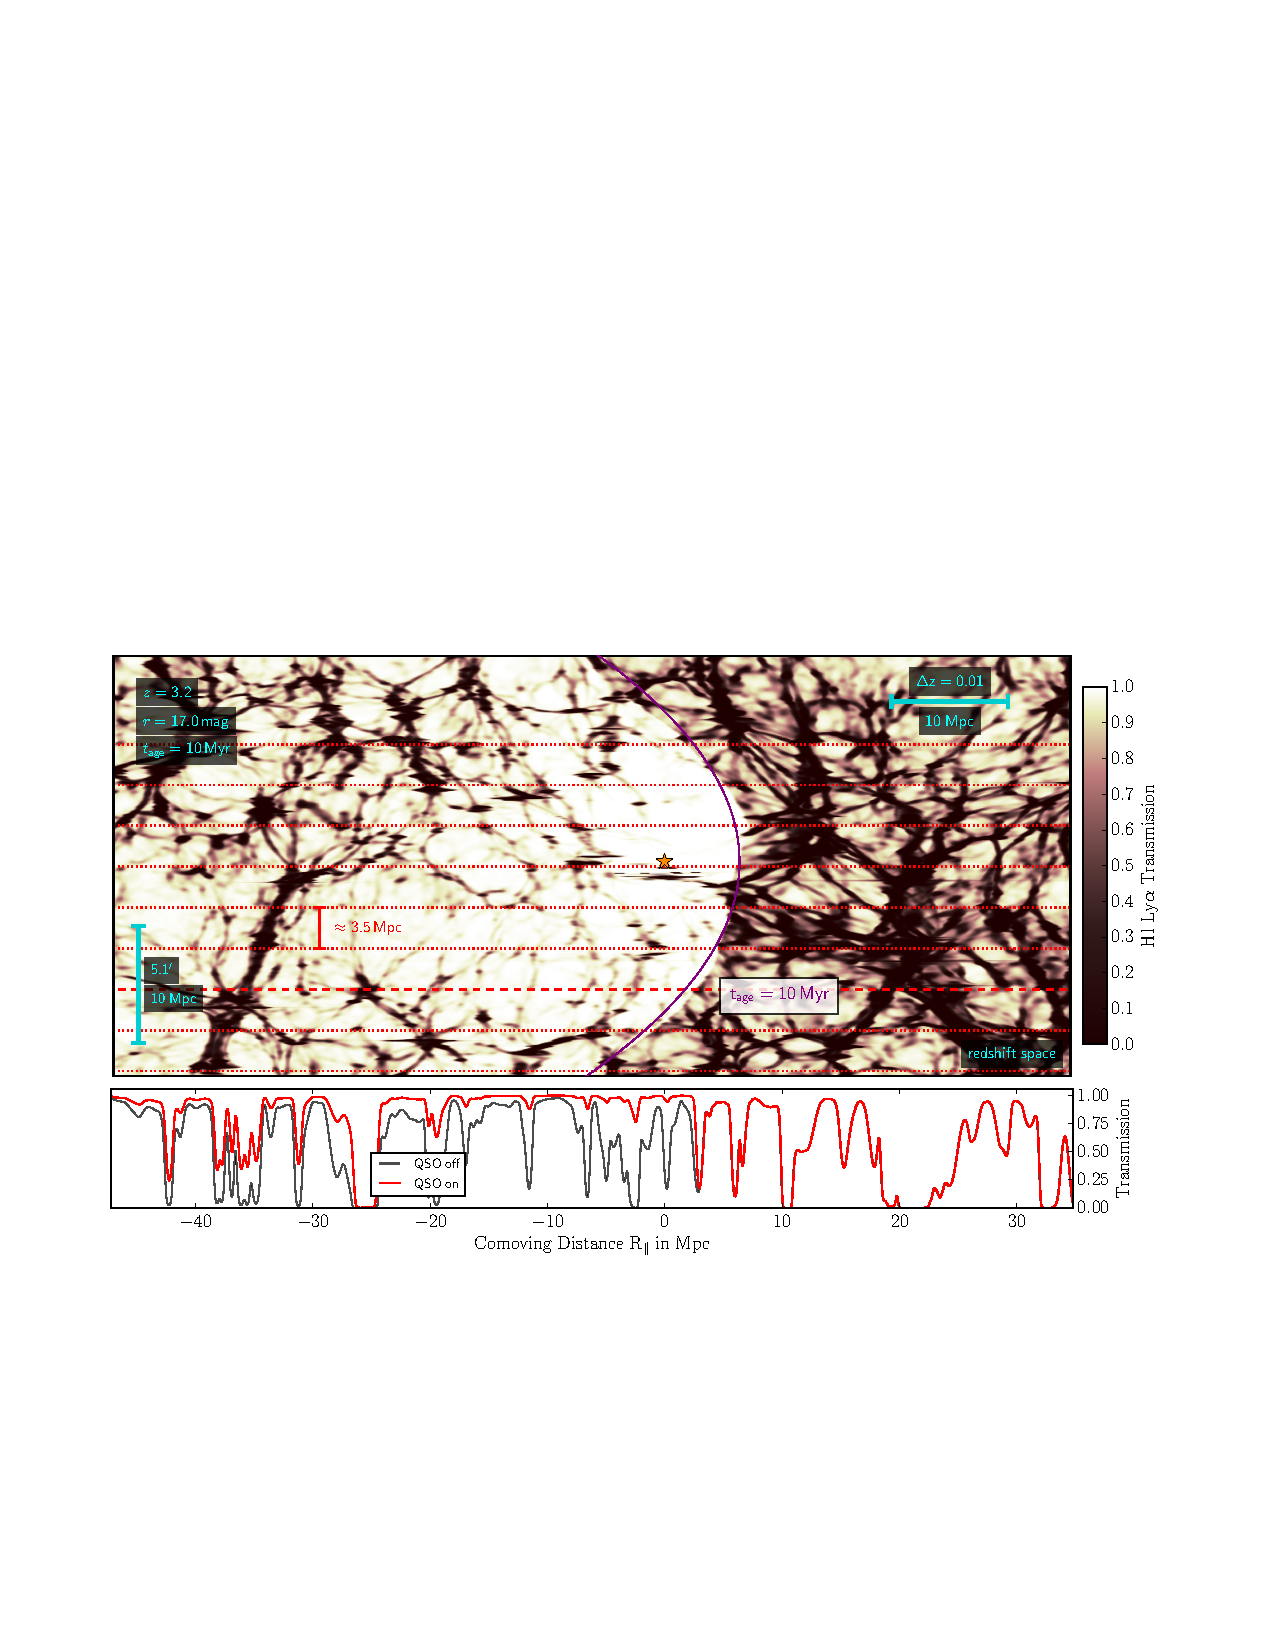
\includegraphics[width=0.6\textwidth]{figs/qso_LightEcho_v1.pdf}
%
\caption{{\it Top}: Quasar ``Light Echos'' revealed in a simulated
tomographic IGM map in the immediate environs of a quasar (gold star)
with several sightlines indicated
\citep[from][]{2018arXiv181005156S}. {\it Bottom}: The ionizing flux
within the echo's extent enhances transmission of Ly$\alpha$ photons
impinging on absorbers along the line-of-sight.}
\label{fig:LightEcho}
\end{wrapfigure}

\subsubsection{Role of environment at $z=1$--$2$ }

Its increased multiplex and high sampling density will allow FOBOS to
map out environmental effects on galaxy evolution at the group scale
($\mathcal{M_\ast/M_\odot} \lesssim 10^{13}$) and, with sufficient
exposure time, for tens of thousands of satellites down to sub-L$^*$
luminosities. Thanks to deep, wide-field imaging surveys, like LSST,
a 1M-object environmental survey at $z=1$--$2$ may then be possible
using improved photo-$z$s, strong priors on spectral types, and new
machine-learning techniques to deliver {\it spectroscopic} redshifts
(with $\lesssim$300 km/s accuracy) at the lowest signal-to-noise
possible (exposure times reduced by factors of 4--5).

%, 2011AJ....142...72E, 2017AJ....154...28B}

% \noindent\comment{Cooper, further comments?}

%\begin{figure}[h!]
%%
%\vskip -0.1in
%%
%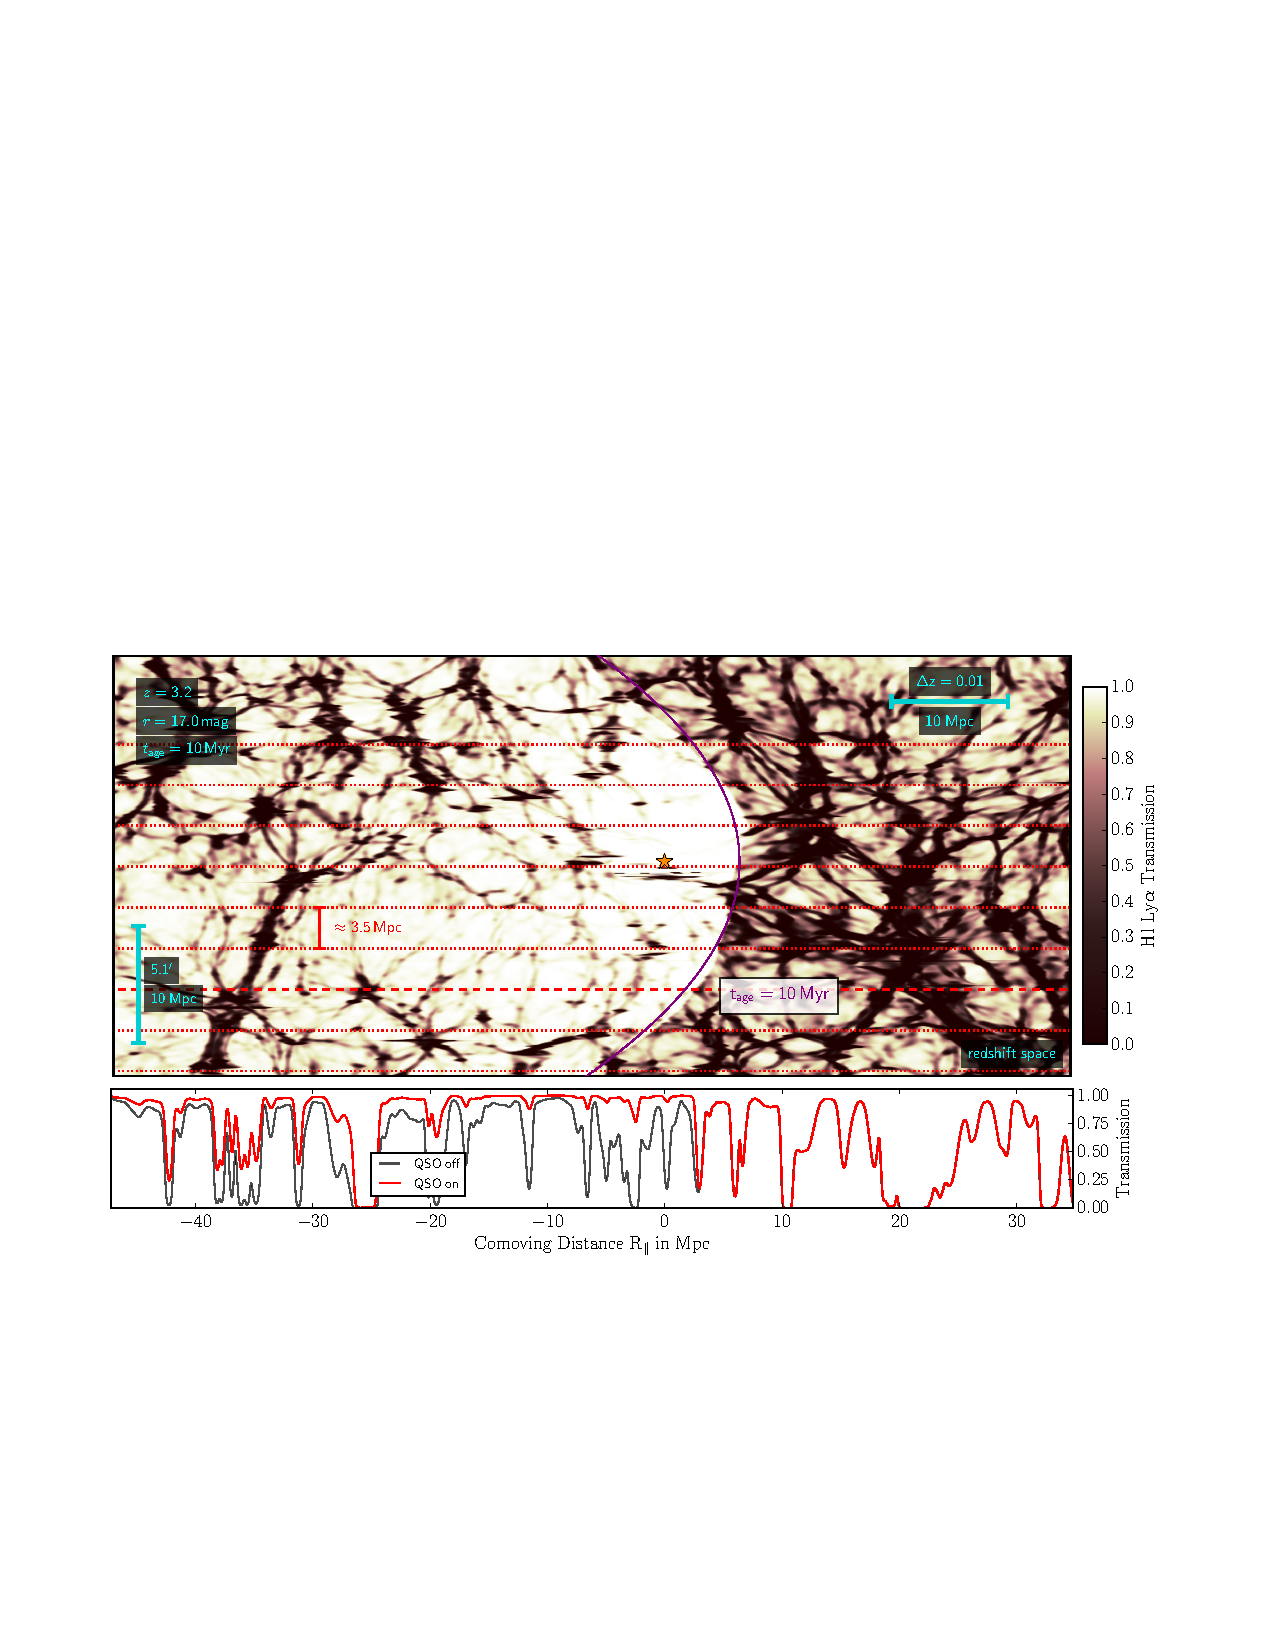
\includegraphics[width=\textwidth]{figs/qso_LightEcho_v1.pdf}
%%
%\caption{{\it Top}: Quasar ``Light Echos'' revealed in a simulated tomographic IGM map in the immediate environs of a quasar (gold star) with several sightlines indicated \citep[from][]{2018arXiv181005156S}.  {\it Bottom}: The ionizing flux within the echo's extent enhances transmission of Ly$\alpha$ photons impinging on absorbers along the line-of-sight.}
%%
%\label{fig:LightEcho}
%%
%\end{figure}

\subsubsection{The $z$$\sim$2 galaxy ecosystem}
\label{sec:z2galaxies}

With surveys like MOSDEF \citep{kriek15} and KBSS
\citep{steidel14}, MOSFIRE has provided powerful new
insights into early galaxies at the $z$$\sim$2 peak-formation epoch.
However, a complete picture of the galaxy ``ecosystem'' at this key
epoch must also consider the gas-filled environments. Using
Ly$\alpha$ absorption in background galaxies, a tomographic map of
the intergalactic medium (IGM) in regions surveyed by MOSDEF and KBSS
is a key first step. The promise of this approach, demonstrated at
Keck by \citet{lee14}, motivates FOBOS's UV sensitivity, target
flexibility, and multiplex for tomographic mapping of large-scale
structure, including protoclusters \citep{lee16}, voids
\citep{krolewski18}, and filaments \citep{horowitz19}.
\citet{2018arXiv181005156S} take IGM tomography in a new direction,
demonstrating with simulated observations that quasar ``light echos''
--- spatial signatures of the expanding ionization front of a newly
activated quasar --- can be detected and used to infer opening angles
and deconstruct the quasar's accretion history (see Fig
\ref{fig:LightEcho}). The required FOBOS spectra can simultaneously
constrain the CIV mass density (via $\lambda\lambda$1548,1550 \AA)
and patterns of CIV enrichment on both IGM and circumgalactic scales,
revealing the imprint of galaxy fueling and feedback processes
\citep[e.g.,][]{tumlinson17}.

%The volume density and chemistry of gas in between galaxies
%\noindent\comment{Hennawi, KG, Prochaska, Burchett: comments? further material to add?}

% \subsection{Ly$\alpha$ morphology and kinematics of lensed, magnified galaxies at $z$$\sim$2--3}

% \noindent\comment{Siana}

% \subsection{The budget of ionizing photons at $z$$\gtrsim$2.5}

% \noindent\comment{Shapley, Siana}


% From George:
% - fill out case for probing both galaxies and their “gas-filled
%   environments”
%    - make it more explicit that getting large numbers of redshifts
%      would make it possible to trace out large-scale structure in
%      detail
%    - enables studies of galaxy properties as a function of environment
%
% - also mention targeting galaxies along QSO lines of sight
%    - much higher target density than with LRIS, DEIMOS over larger FOV.
%
% - Worth discussing Lyman-alpha or metal-line tomography?  
%
% - More quantitative comparisons with existing data sets?
%    - What key science questions can FOBOS address that many years of
%      LRIS and DEIMOS observations have not been able to?  Surely some
%      level of the spectral tagging and photo-z training can be done
%      (and surely is being done) with existing data.  Is FOBOS going to
%      be a huge leap, or will it mainly be cleaning up neglected corners
%      of parameter space?
%
% - More excited to hear about how the FOBOS spectra will be used for
%   science directly, instead of support for LSST

%-----------------------------------------------------------------------

%%%%
% -- Cosmology Science
% --     FOBOS Keck White Paper 2019
%%%%

%\begin{wrapfigure}{r}{0.55\textwidth} %
%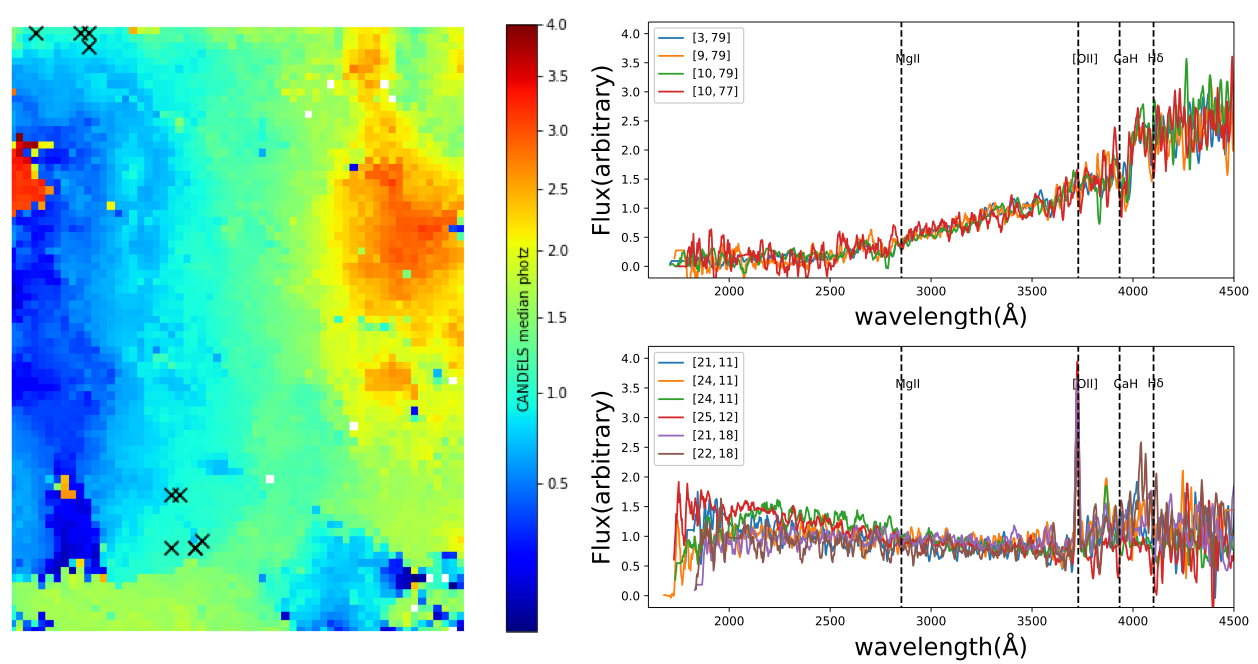
\includegraphics[width=0.55\textwidth]{figs/Hemmati18_Fig8_VVDS_spec.png}
%\caption{\small {\it Left}: A Self-Organizing Map
%\citep[SOM;][]{1990Natur.346...24K} from \citet{hemmati18} relating
%LSST+WFIRST-like galaxy colors to redshift, $z$. FOBOS spectroscopic
%training samples can be optimally designed to populate/calibrate
%sparsely sampled regions. {\it Right}: Galaxy spectra from VVDS
%\citep{2005A&A...439..845L} in SOM locations marked by black crosses.
%More than just redshifts, the detailed similarity of spectral
%features of galaxies localized within the SOM demonstrates
%higher-level inferences (e.g. SFR) are possible given appropriate
%training samples from FOBOS.} \label{fig:SOM} \end{wrapfigure}

\subsection{Dramatically Enhancing Cosmological Probes}

\subsubsection{Dark Energy Probes via Precision Cosmic Distances.}
\label{sec:cosmology}

Panoramic imaging surveys (e.g., LSST, Euclid, and WFIRST) are seeking to constrain the dark-energy
equation-of-state at $z \lesssim 1$ through measurements of angular correlations of galaxy positions, their
gravitational lensing shear, and the cross-correlation between the two.  These surveys rely on photometric redshifts
(``photo-$z$s''), whose uncertainties and potential biases are the major limitation and source of systematic error in
these efforts.  \citet{newman15} define a \emph{spectroscopic} survey for photo-$z$ training that would \emph{increase
the dark energy figure-of-merit in LSST by 40\%}.  The survey program is ideally matched to FOBOS.  It requires 10
independent fields, each 20 arcmin in diameter, with a sampling density of 6 arcmin$^{-2}$, and the ability to go very
deep ($i_{\rm AB} < 25.3$).  FOBOS's lack of a ``redshift desert'' further eliminates the need for expensive, space-based\footnote{Ground-based near-IR spectroscopy is too contaminated by
sky-line emission to provide spec-$z$s at the required level of completeness \citep{newman15}.} near-IR spectroscopy to train photo-$z$s with $z > 1.5$.  Highly accurate photo-$z$s will enable science applications that go beyond cosmology.

\subsubsection{Cosmology with LBG--CMB cross correlation.}
\label{sec:LBG}

High-S/N CMB maps from next-generation CMB observatories (e.g., Simons Observatory and CMB-S4) will provide a cosmic
``reference background'' for measurements of gravitational lensing induced by matter along the line of sight.  After
cross-correlating with Lyman Break Galaxy (LBG) samples, a relatively flat lensing ``kernel'' with power at $z = 2$--5
enables powerful constraints on the Inflation-sensitive matter power spectrum, Horizon-scale General Relativity, cosmic
curvature and neutrino masses, and early Dark Energy.  \citet{wilson19} explore these constraints in detail and
highlight the need for spectroscopic determination of accurate redshift distributions for the employed LBG samples.
FOBOS would address this need in two ways.  First, several deep-drilling fields targeting $\sim$1000 LBGs BX, $u$, $g$,
and $r$ drop-out candidates per pointing ($\sim$10,000 deg$^{-2}$) would establish the interloper rate and intrinsic
redshift distribution of LBG samples to sufficient precision (this program would likely overlap with the photo-$z$
program described above).  Second, $\sim$200 LBGs per pointing (2000 deg$^{-2}$) could be included as a background
program when FOBOS observes other sources across the sky, eventually building a 50-100 deg$^2$ data set of sparse
high-$z$ spectroscopy for LBG dN/d$z$ calibration via clustering redshifts \citep[see][]{wilson19}.


% \subsection{Kinematic weak lensing.}
% \label{sec:kinematic_lensing}

% Kinematic weak lensing is a promising new technique that measures shear in projected velocity fields of source galaxies to infer the presence of mass along the line-of-sight.  While compared to traditional photometric lensing, kinematic lensing requires more expensive resolved spectroscopy, it also yields shear measurements with 10 times the S/N per source galaxy \citep{huff13}.  This is because the result of velocity field lensing is uniquely defined whereas photometric lensing depends on the (unknown) intrinsic shape and orientation of the galaxy.  The kinematic lensing observable can be expressed as the offset between the kinematic major axis position angle (PA) and the photometric PA.  Small, 7-fiber IFU bundles can measure kinematic PAs to $\sim$1 degree precision (DiGiorgio in prep.), motivating a FOBOS deployment of 250 such IFUs per field that could measure mass profiles of galaxy cluster halos, perform targeted galaxy-galaxy lensing experiments, or provide checks on cosmological photometric lensing results from surveys like LSST.  Further work on developing this science case is underway. 




%%%%
% -- Data Science
% --     FOBOS Keck White Paper 2019
%%%%

% \begin{wrapfigure}{r}{0.55\textwidth} %
% 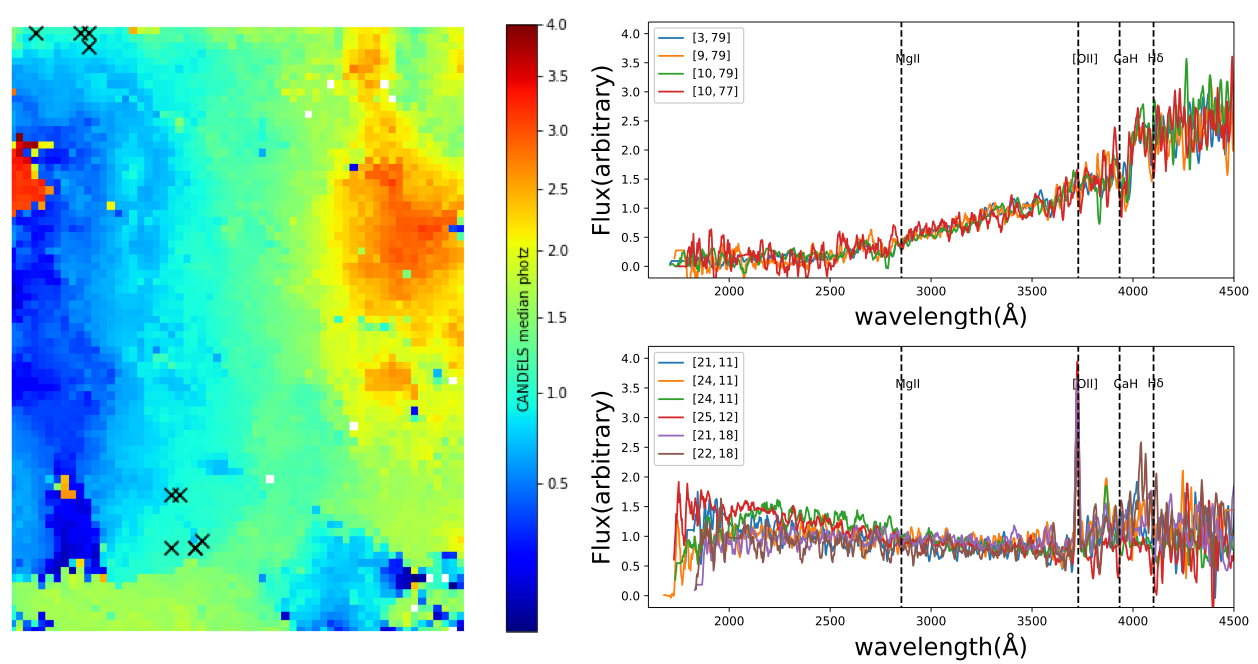
\includegraphics[width=0.55\textwidth]{figs/Hemmati18_Fig8_VVDS_spec.png}
% \caption{\small {\it Left}: A Self-Organizing Map
% \citep[SOM;][]{1990Natur.346...24K} from \citet{hemmati18} relating
% LSST+WFIRST-like galaxy colors to redshift, $z$. FOBOS spectroscopic
% training samples can be optimally designed to populate/calibrate
% sparsely sampled regions. {\it Right}: Galaxy spectra from VVDS
% \citep{2005A&A...439..845L} in SOM locations marked by black crosses.
% More than just redshifts, the detailed similarity of spectral
% features of galaxies localized within the SOM demonstrates
% higher-level inferences (e.g. SFR) are possible given appropriate
% training samples from FOBOS.} \label{fig:SOM} \end{wrapfigure}


\subsection{FOBOS as an ideal spectroscopic training instrument}
\label{sec:datascience}

In all three science areas above, FOBOS offers significant advances by serving as the leading U.S.~facility in providing  
spectroscopic \emph{training} data. As machine learning
techniques advance in the coming decade, spectroscopic ``training''
as a means of extracting the maximum information from billions of
photometric sources across thousands of deg$^2$ becomes increasingly
important. The required training samples at LSST
depths will fill even the modest Keck focal plane with 10's of
thousands of sources. The key requirements are sensitivity and
multiplex (not field-of-view). Emphasizing these, FOBOS will be an
ideal training facility for LSST-era photometric redshifts
\citep[see][]{salvato19}, galaxy physical properties
\citep[e.g.,][]{davidzon19}, and stellar parameters
\citep[e.g.,][]{2018arXiv180401530T}.

% Above, we have focused on specific studies that directly benefit from
% FOBOS's capabilities. However, FOBOS will also allow teams of Keck
% scientists to quickly build spectoscopic samples purposely designed
% to be used as spectroscopic training sets. Here, we highlight two
% cases where well-designed FOBOS observations can be used in novel
% machine-learning applications.

% These data will allow us to statistically infer physical properties
% from upcoming large-scale broad-band imaging surveys (e.g., LSST,
% WFIRST, Euclid) that are only directly accessible via spectroscopy
% and complement more shallow spectroscopic surveys made with FOBOS or
% surveys using smaller aperture facilities (e.g., APOGEE, DESI).
% Keying off one of NSF's ten Big Ideas, we highlight a few ways that
% FOBOS can be used to "harness the data revolution."

% \begin{figure}[h!]
% \vskip -0.1in
% 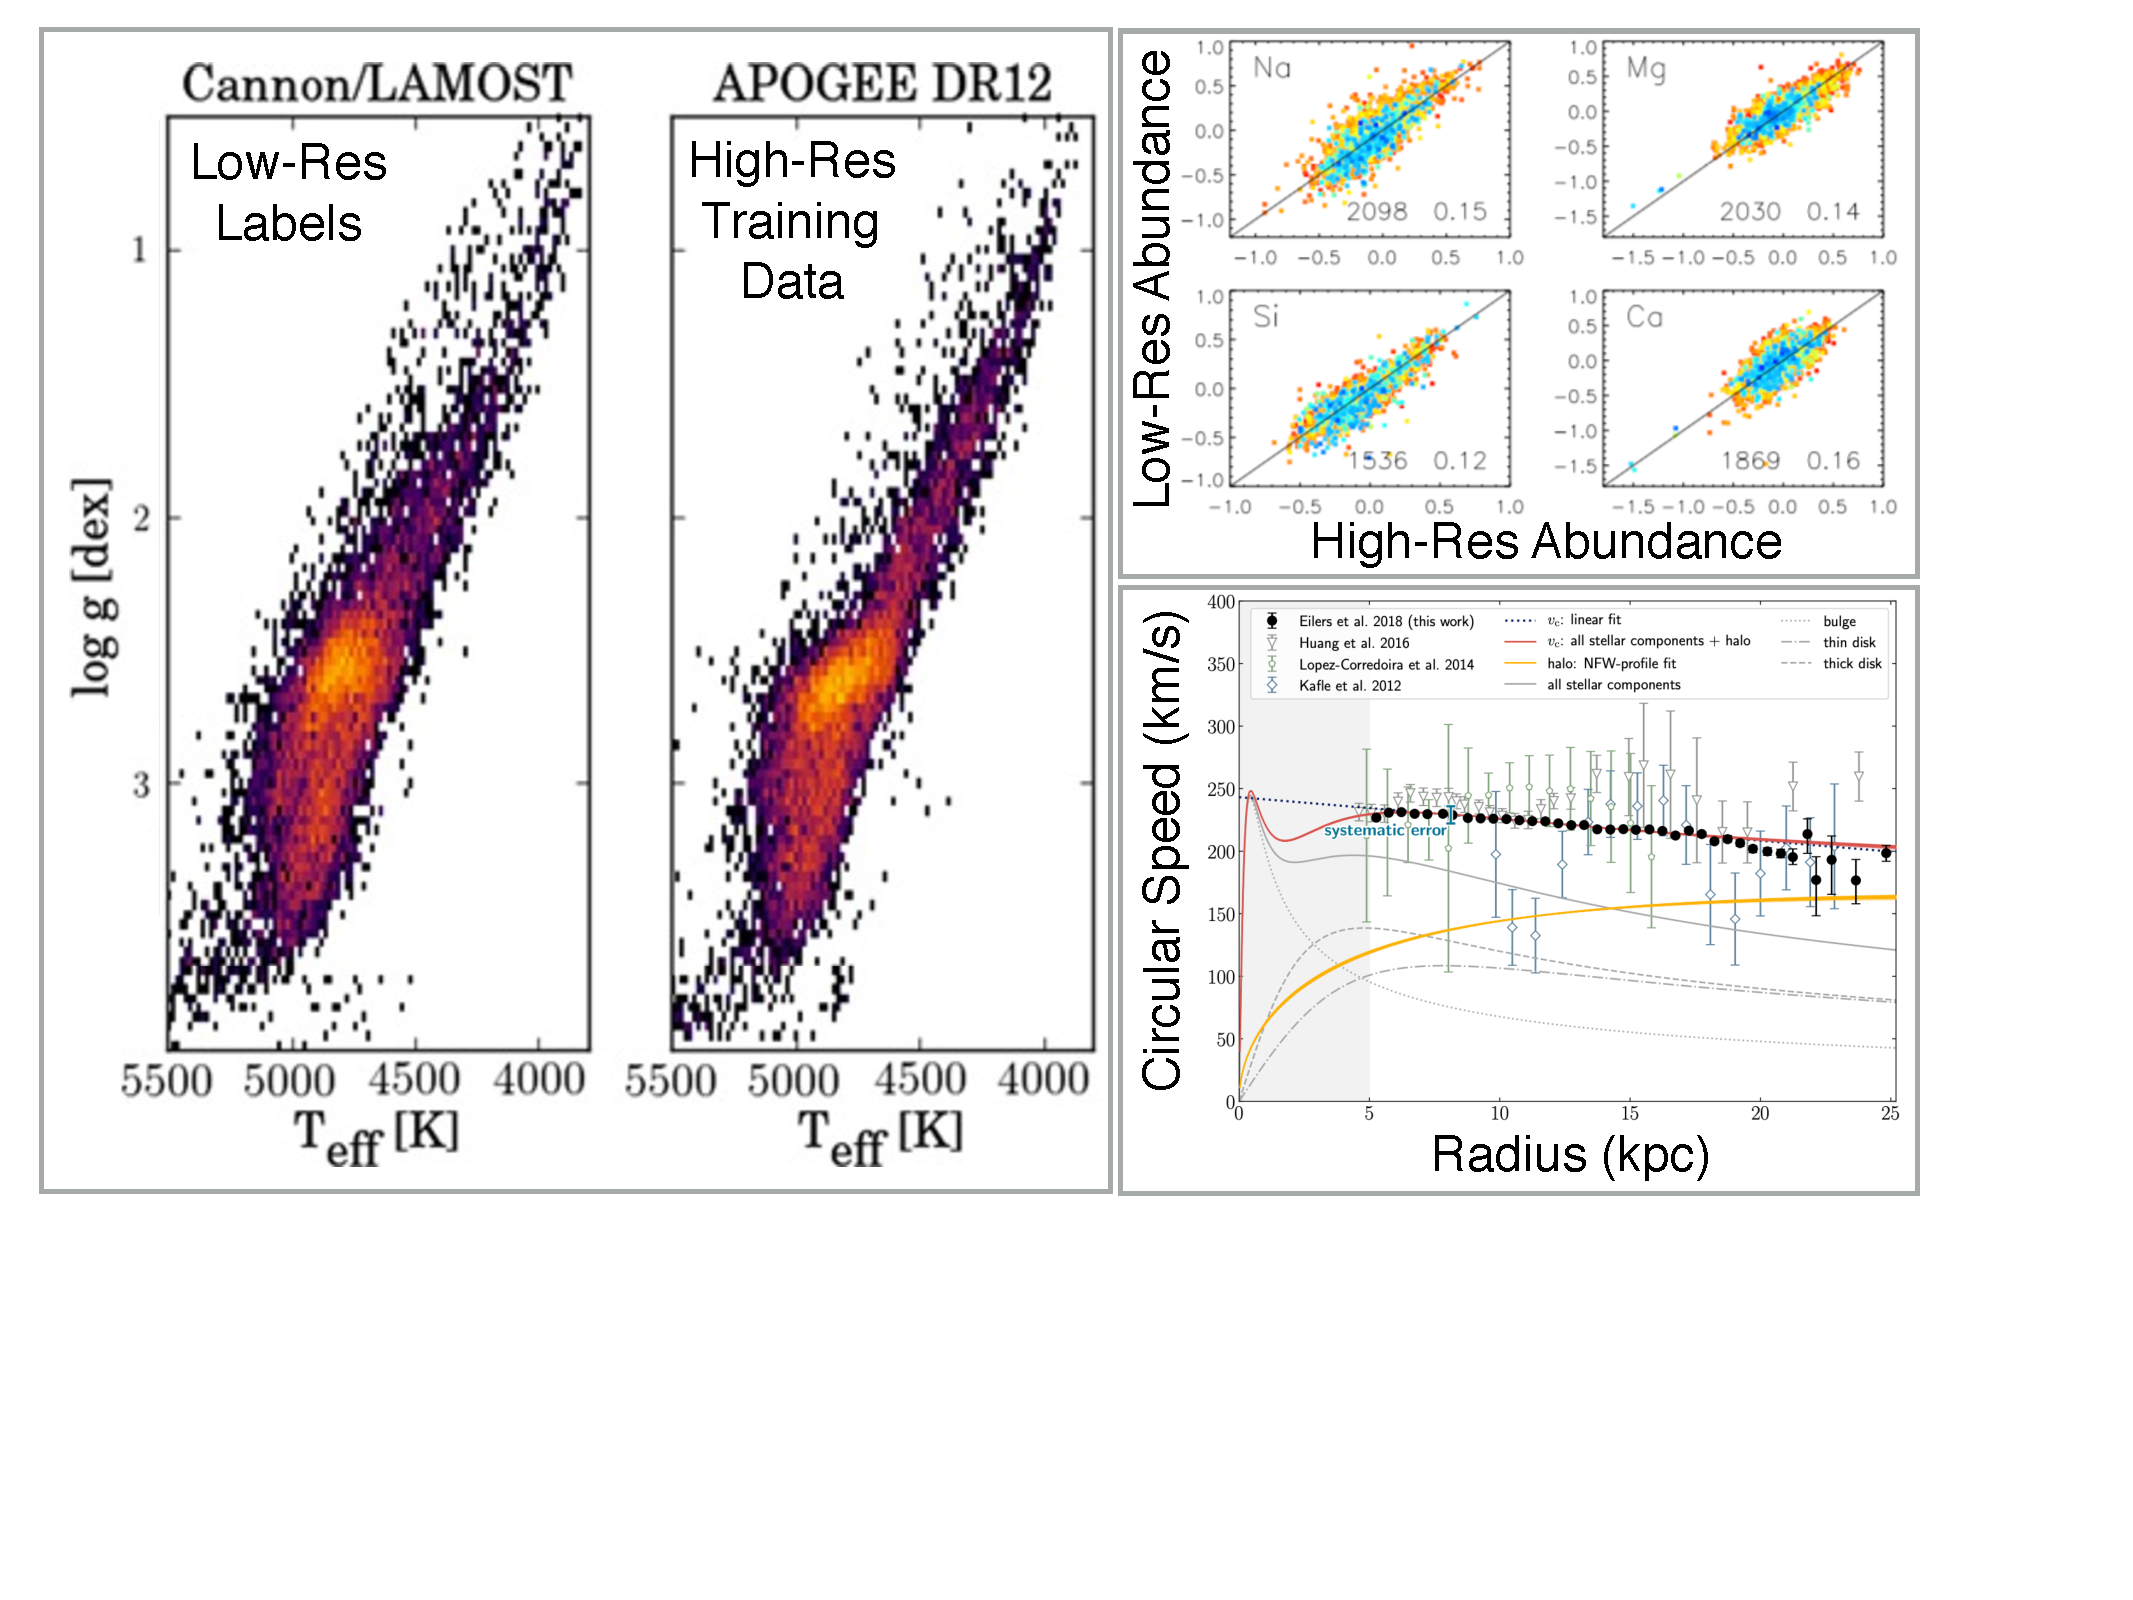
\includegraphics[width=\textwidth]{figs/LGplots.pdf}
% \caption{{\it Left}: Validation of {\it The Cannon} measurements of
% stellar effective temperature, $T_{\rm eff}$, and surface gravity,
% $\log g$, using low-resolution LAMOST spectra (left) compared to
% high-resolution APOGEE measurements
% \citep[right;][]{2017ApJ...836....5H}. {\it Top-right}: Recovery of
% elemental abundances from low-resolution LAMOST spectra compared to
% high-resolution measurements from GALAH (Xiang et al., in prep). {\it
% Bottom-right}: The circular-speed curve of the Milky Way determined
% using a data-driven model that combines stellar parameters determined
% from APOGEE spectra with photometry from WISE, 2MASS, and Gaia
% \citep{2019ApJ...871..120E}. FOBOS will be a premier instrument for
% such machine-learning applications.}
% \label{fig:Cannon}
% \end{figure}

% \subsubsection{The chemical evolution of Milky Way stellar
% populations} Kinematics and chemical-abundance measurements for stars
% in the MW halo or the M31 disk require observations of 10 hours or
% more on large telescopes \citep[e.g.,][]{2018arXiv180904082C}.
% However, machine-learning algorithms can be used to extract physical
% quantities from both multi-band imaging and lower quality spectra
% (low resolution and S/N) using relatively small, high-S/N, training
% sets (e.g., Fig.~\ref{fig:Cannon}). The goal of such applications is
% to reach magnitudes significantly fainter than the detection limit of
% current and upcoming spectroscopic surveys by designing an optimized,
% nested set of FOBOS training samples. This nested set will vary in
% S/N and spectral resolution for sufficiently large, overlapping
% stellar samples, and include astroseismology from TESS and PLATO for
% some subset. Within this nested set, low-resolution FOBOS data will
% fill gaps at both high-S/N, where we can train FOBOS data on
% higher resolution spectroscopy, and low-S/N, where we will
% be training photometry on FOBOS spectroscopy. The success of this
% multi-layered inference depends not only on the size of the training
% sets we can access or observe, but on how representative they are.
% For example, inference of M31 halo stellar properties from WFIRST
% photometry based on a MW-trained set of FOBOS spectroscopy will
% require accuracy assessments using simulated data.

% For example, \citet{2015ApJ...808...16N} have developed {\it The
% Cannon}, a supervised learning approach that uses spectra with known
% stellar parameters to label spectra where those parameters are
% unknown (Fig.~\ref{fig:Cannon}). Additionally,
% \citet{2018arXiv180401530T} have developed {\it The Payne} which can
% infer 16 stellar-abundance labels from low-resolution spectra using a
% neural network and theoretical stellar spectra. Finally,
% \citet{2018arXiv180803278T} have combined Kepler-based
% astroseismology measurements with APOGEE spectra to determine stellar
% age to $\sim$25\% precision using a neural network. Our proposed
% effort builds on new lines of inquiry based on these successes.

% of the Milky Way including Gaia, APOGEE, the SDSS-V Milky Way Mapper,
% planned programs with 4MOST and the Dark Energy Spectroscopic
% Instrument (DESI) Milky Way Survey, among others. Inferring stellar
% parameters beyond $V$$\sim$18 will open up studies of the Milk Way’s
% outer halo, the halo of M31, and stellar populations in local dwarf
% galaxies.

% Using simulated spectra with known input parameters, we will test
% methods for ``label transfer'' from information-rich spectra to
% information-poor spectra as we work down to fainter magnitudes,
% landing eventually at multi-band photometry alone.

% We will test it by evaluating label recovery on simulated stellar
% spectra with cosmologically-informed formation histories for M31 and
% dwarf galaxies, suitably differentiated from the Milky Way stars that
% anchor the training network.

% \subsubsection{The $z$$\sim$2 Galaxy Population}

% \begin{figure}[h!]
% \vskip -0.1in
% 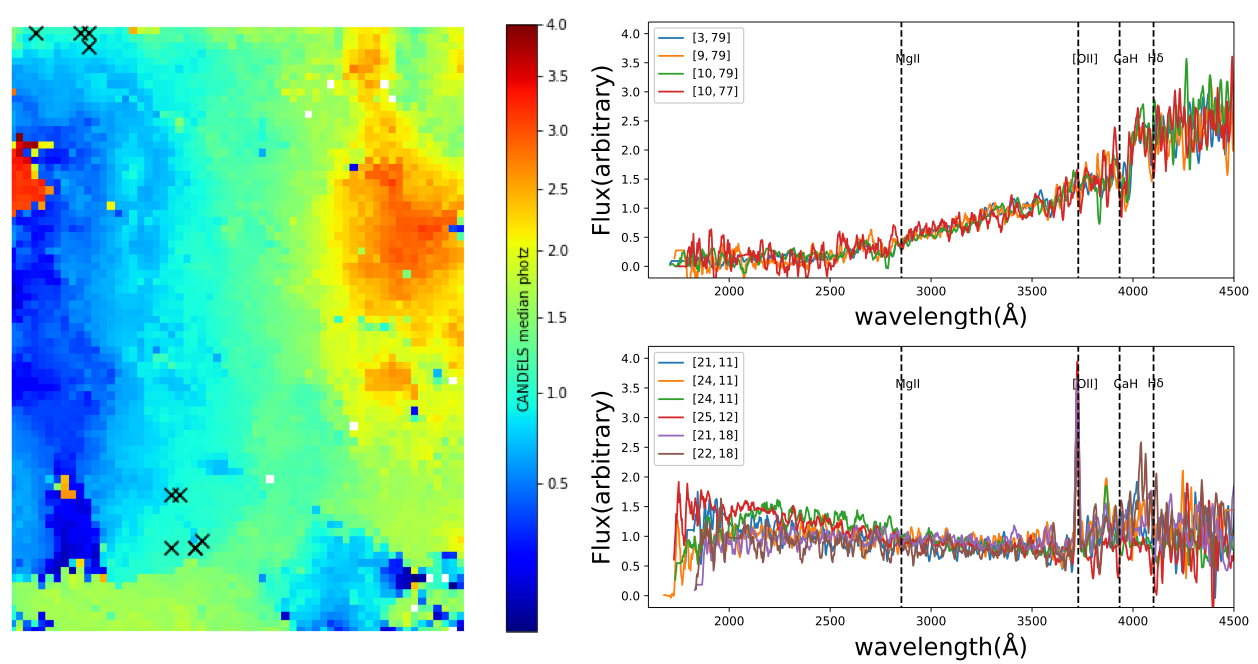
\includegraphics[width=\textwidth]{figs/Hemmati18_Fig8_VVDS_spec.png}
% \caption{\small {\it Left}: A Self-Organizing Map
% \citep[SOM;][]{1990Natur.346...24K} from \citet{hemmati18}, which
% encodes the relation between galaxy colors in an LSST+WFIRST-like
% color space and their redshift, $z$. Such SOMs can be used to
% optimally define FOBOS spectroscopic training samples for use with
% imaging surveys to populate sparsely sampled regions. {\it Right}:
% Galaxy spectra from VVDS \citep{2005A&A...439..845L}; black crosses
% near the top and bottom of the SOM are plotted in the top and bottom
% panels, respectively. The detailed similarity of spectral features of
% galaxies localized within the SOM suggests a systematic spectroscopic
% exploration with FOBOS of the LSST color space allows for inference
% of galaxy physical properties beyond a photo-$z$ training
% application.}
% \label{fig:SOM}
% \end{figure}

% % Galaxies observed in this space are assigned $z$ values based on the
% % median photo-$z$ of galaxies from the CANDELS survey \citep[color
% % bar;][]{2011ApJS..197...35G}.

% For decades, we have used the spectral information encoded in
% broad-band photometry to infer properties of galaxies beyond their
% color and brightness. The most common application is to estimate the
% galaxy redshift, i.e. photometric redshifts (photo-$z$s). However, a
% range of observed spectral features are well-constrained by
% broad-band imaging (Fig. \ref{fig:SOM}), suggesting a far greater
% potential for imaging data to reveal physical properties with
% sufficient training of deep-learning algorithms. Self-Organizing Maps
% (SOM, Figure \ref{fig:SOM}) provide a state-of-the-art representation
% of a high-dimensional input space in projected 2D grid cells,
% allowing us to benchmark sampling of the photometric color space
% under various training set designs. The compelling prospect of this
% approach is its utility in delivering SDSS-like information --- e.g.,
% star-formation histories, stellar-population properties, dust
% content, inflow/outflow properties, and stellar masses --- for
% the millions of galaxies imaged by LSST at $z$$\sim$2.

% These properties go beyond what conventional modeling of spectral
% energy distributions (SEDs) would suggest.

% We will also use Bayesian Optimization techniques to evaluate the
% success of simulated training sets against the fidelity of full
% cosmological analyses that employ them. This will enable extremely
% rapid exploration of the optimal design space.

%\comment{Masters, Mandelbaum, Rau, Schafer}

% The complete photo-$z$ training survey described in \citet{newman15}
% would require 15 independent pointings, each spanning 0.1 deg$^2$ with
% a target density of 6 arcmin$^{-2}$ (8 arcmin$^{-2}$ when including $z
% > 1.5$ galaxies accessible in the UV with Keck-FOBOS), perfectly
% matched to the Keck-FOBOS field-of-view and target density.  With a
% conservative exposure time of 100 hours to reach 75\% redshift
% completeness for 40,000 galaxies with $i_{\rm AB} < 25.3$, the Neman
% survey would require 400 nights.  Challenge \ref{photoz} would reduce
% the required survey duration by a factor of at least four.  Meanwhile
% the extreme depths and flux-limited selection are likely also
% requirements for training sets associated with Challenges \ref{phot},
% \ref{uv}.

% A wider and shallower survey component is envisioned for Challenges
% \ref{lowsnr} and \ref{gaia}.  With 10-minute integrations, a 52
% deg$^2$ Keck-FOBOS sample of environmental diagnostics for 1 million
% galaxies could be carried out in less than 20 nights.  This program
% would sample at $z \sim 1.5$ the same cosmic volume as SDSS.  A
% program of a similar scale would provide training set data for
% inference of stellar parameters in the Milky Way.  These shallow
% programs would be integrated with the deeper components described
% above into a single survey plan.



%%%%
% -- Instrument Description
% --     FOBOS Keck White Paper 2019
%%%%

%%%%%%%%%%%%%%%%%%%%%%%%%%%%%%%%%%%%%%%%%%%%%%%%%%%%%%%%%%%%%%%%%%%%%%%%
\begin{figure}[h!]
%\vskip -0.1in
%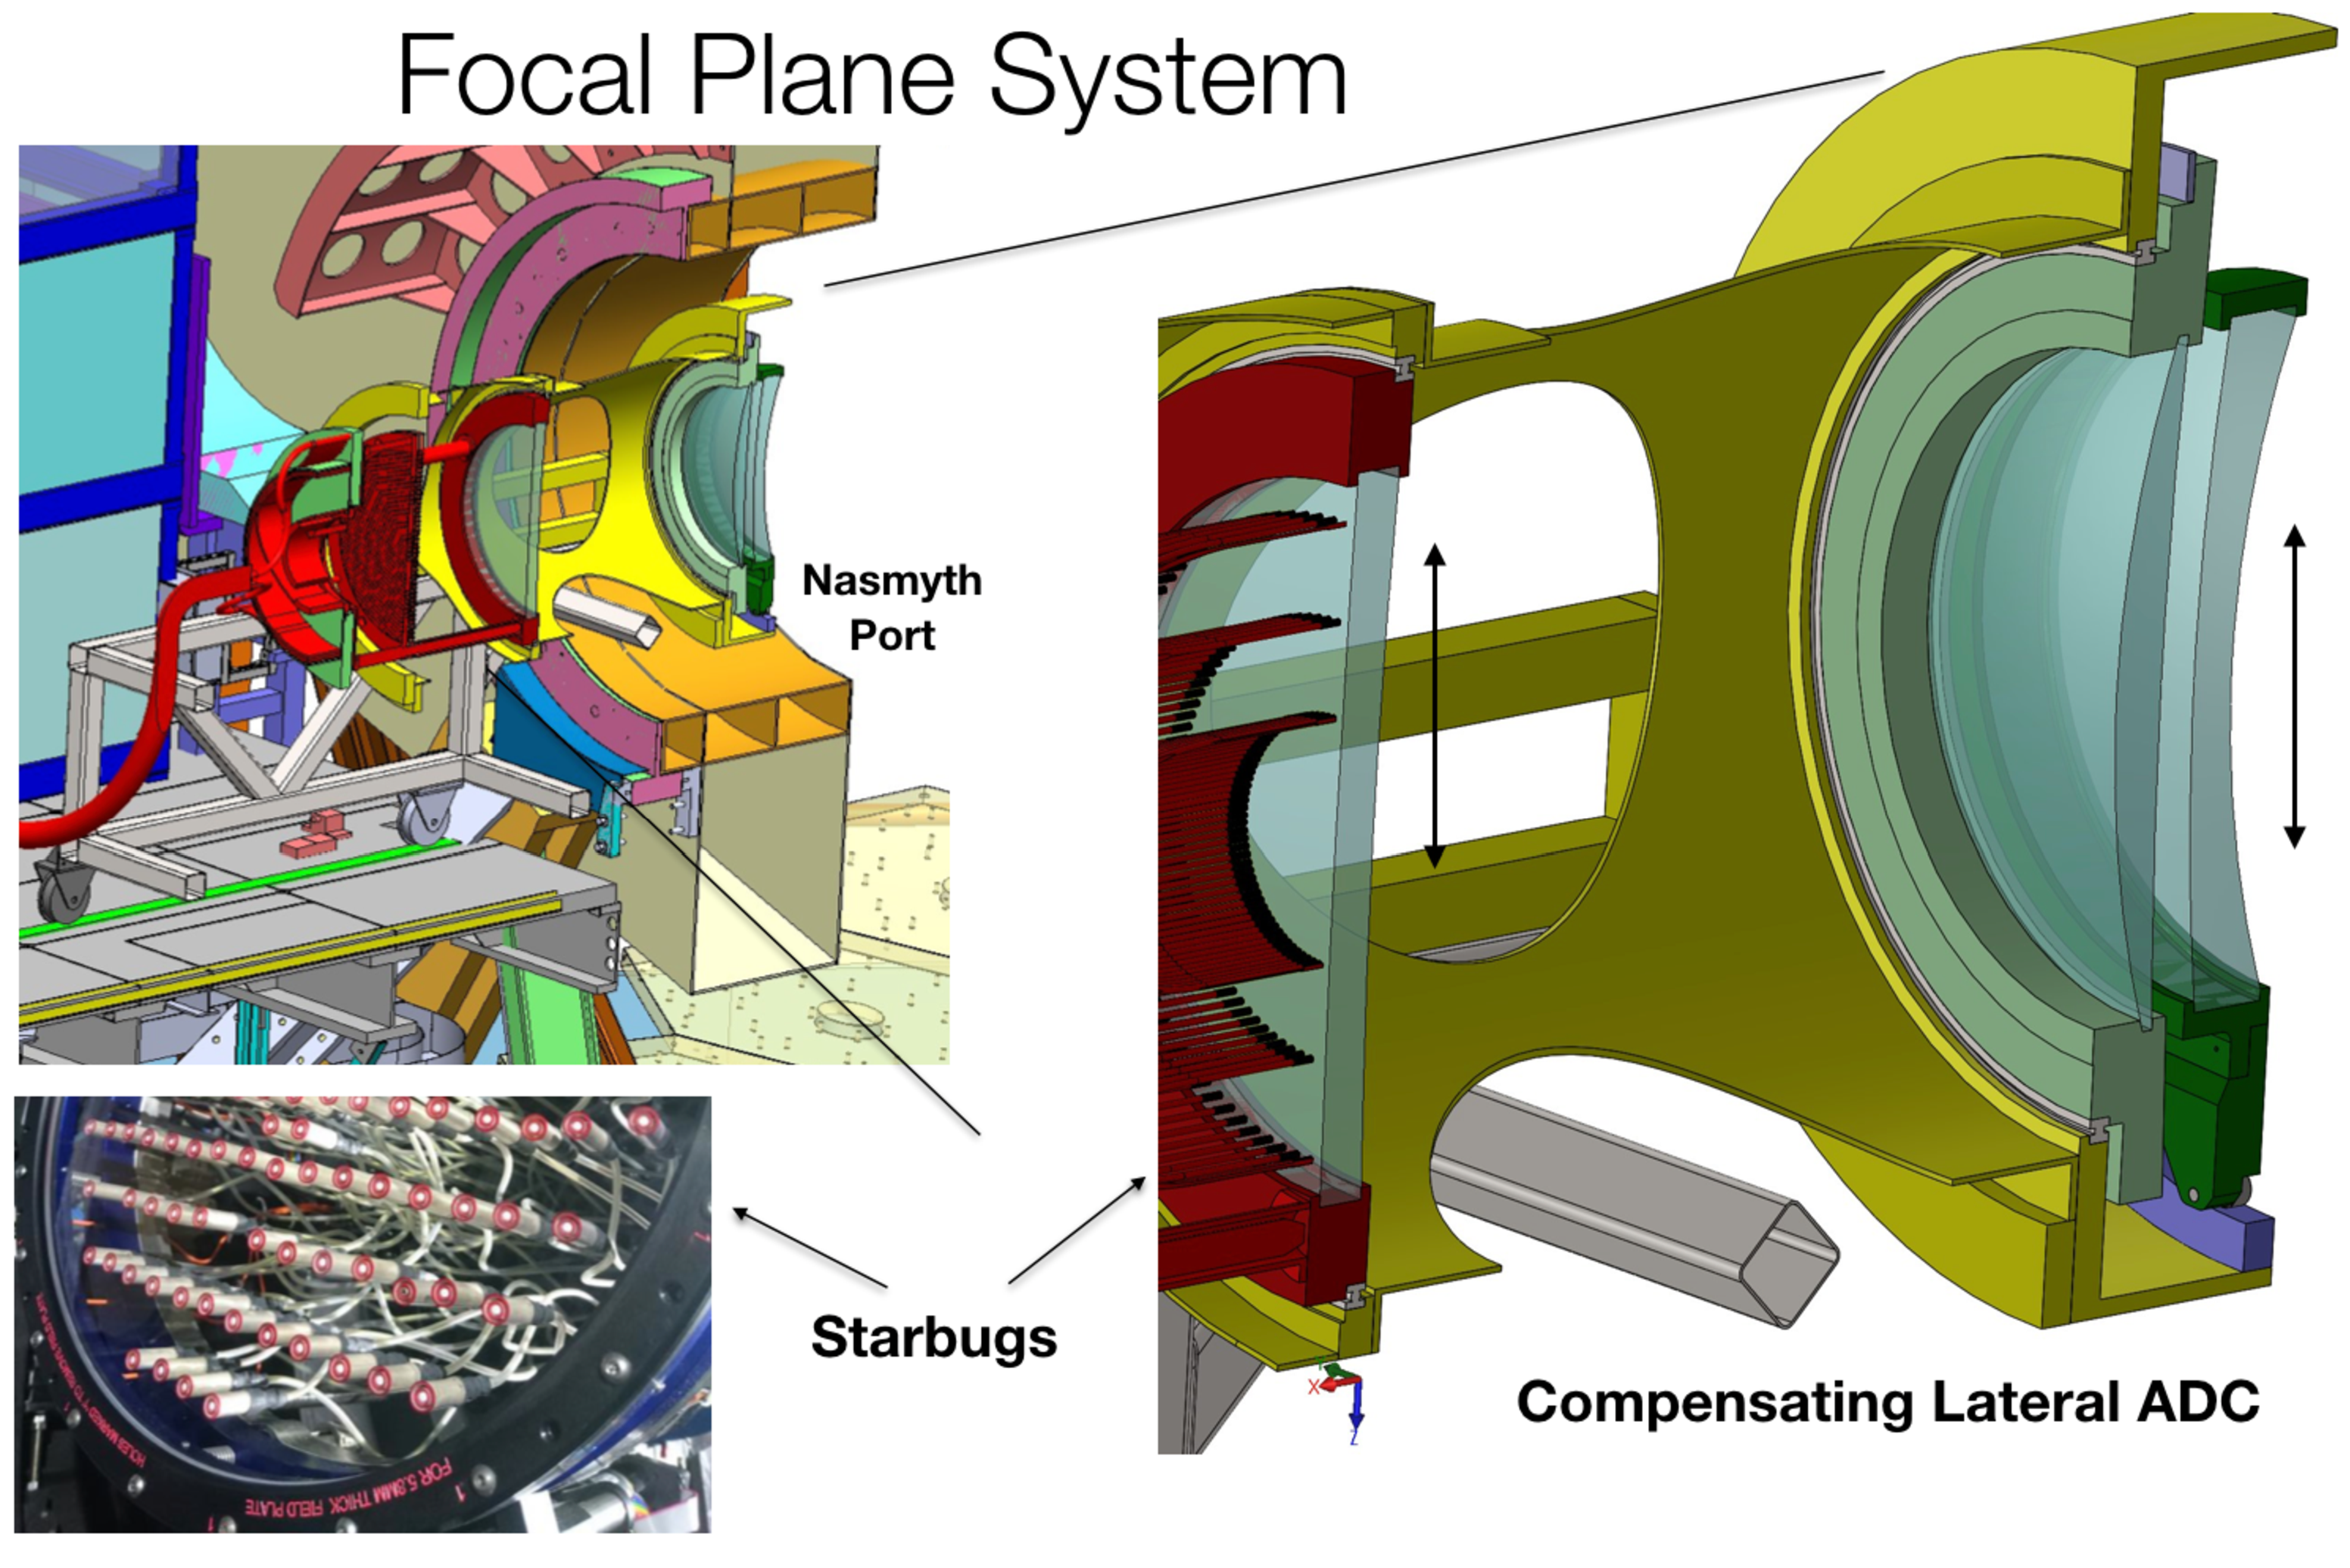
\includegraphics[width=\textwidth]{figs/FOBOS_FocalPlane.pdf}
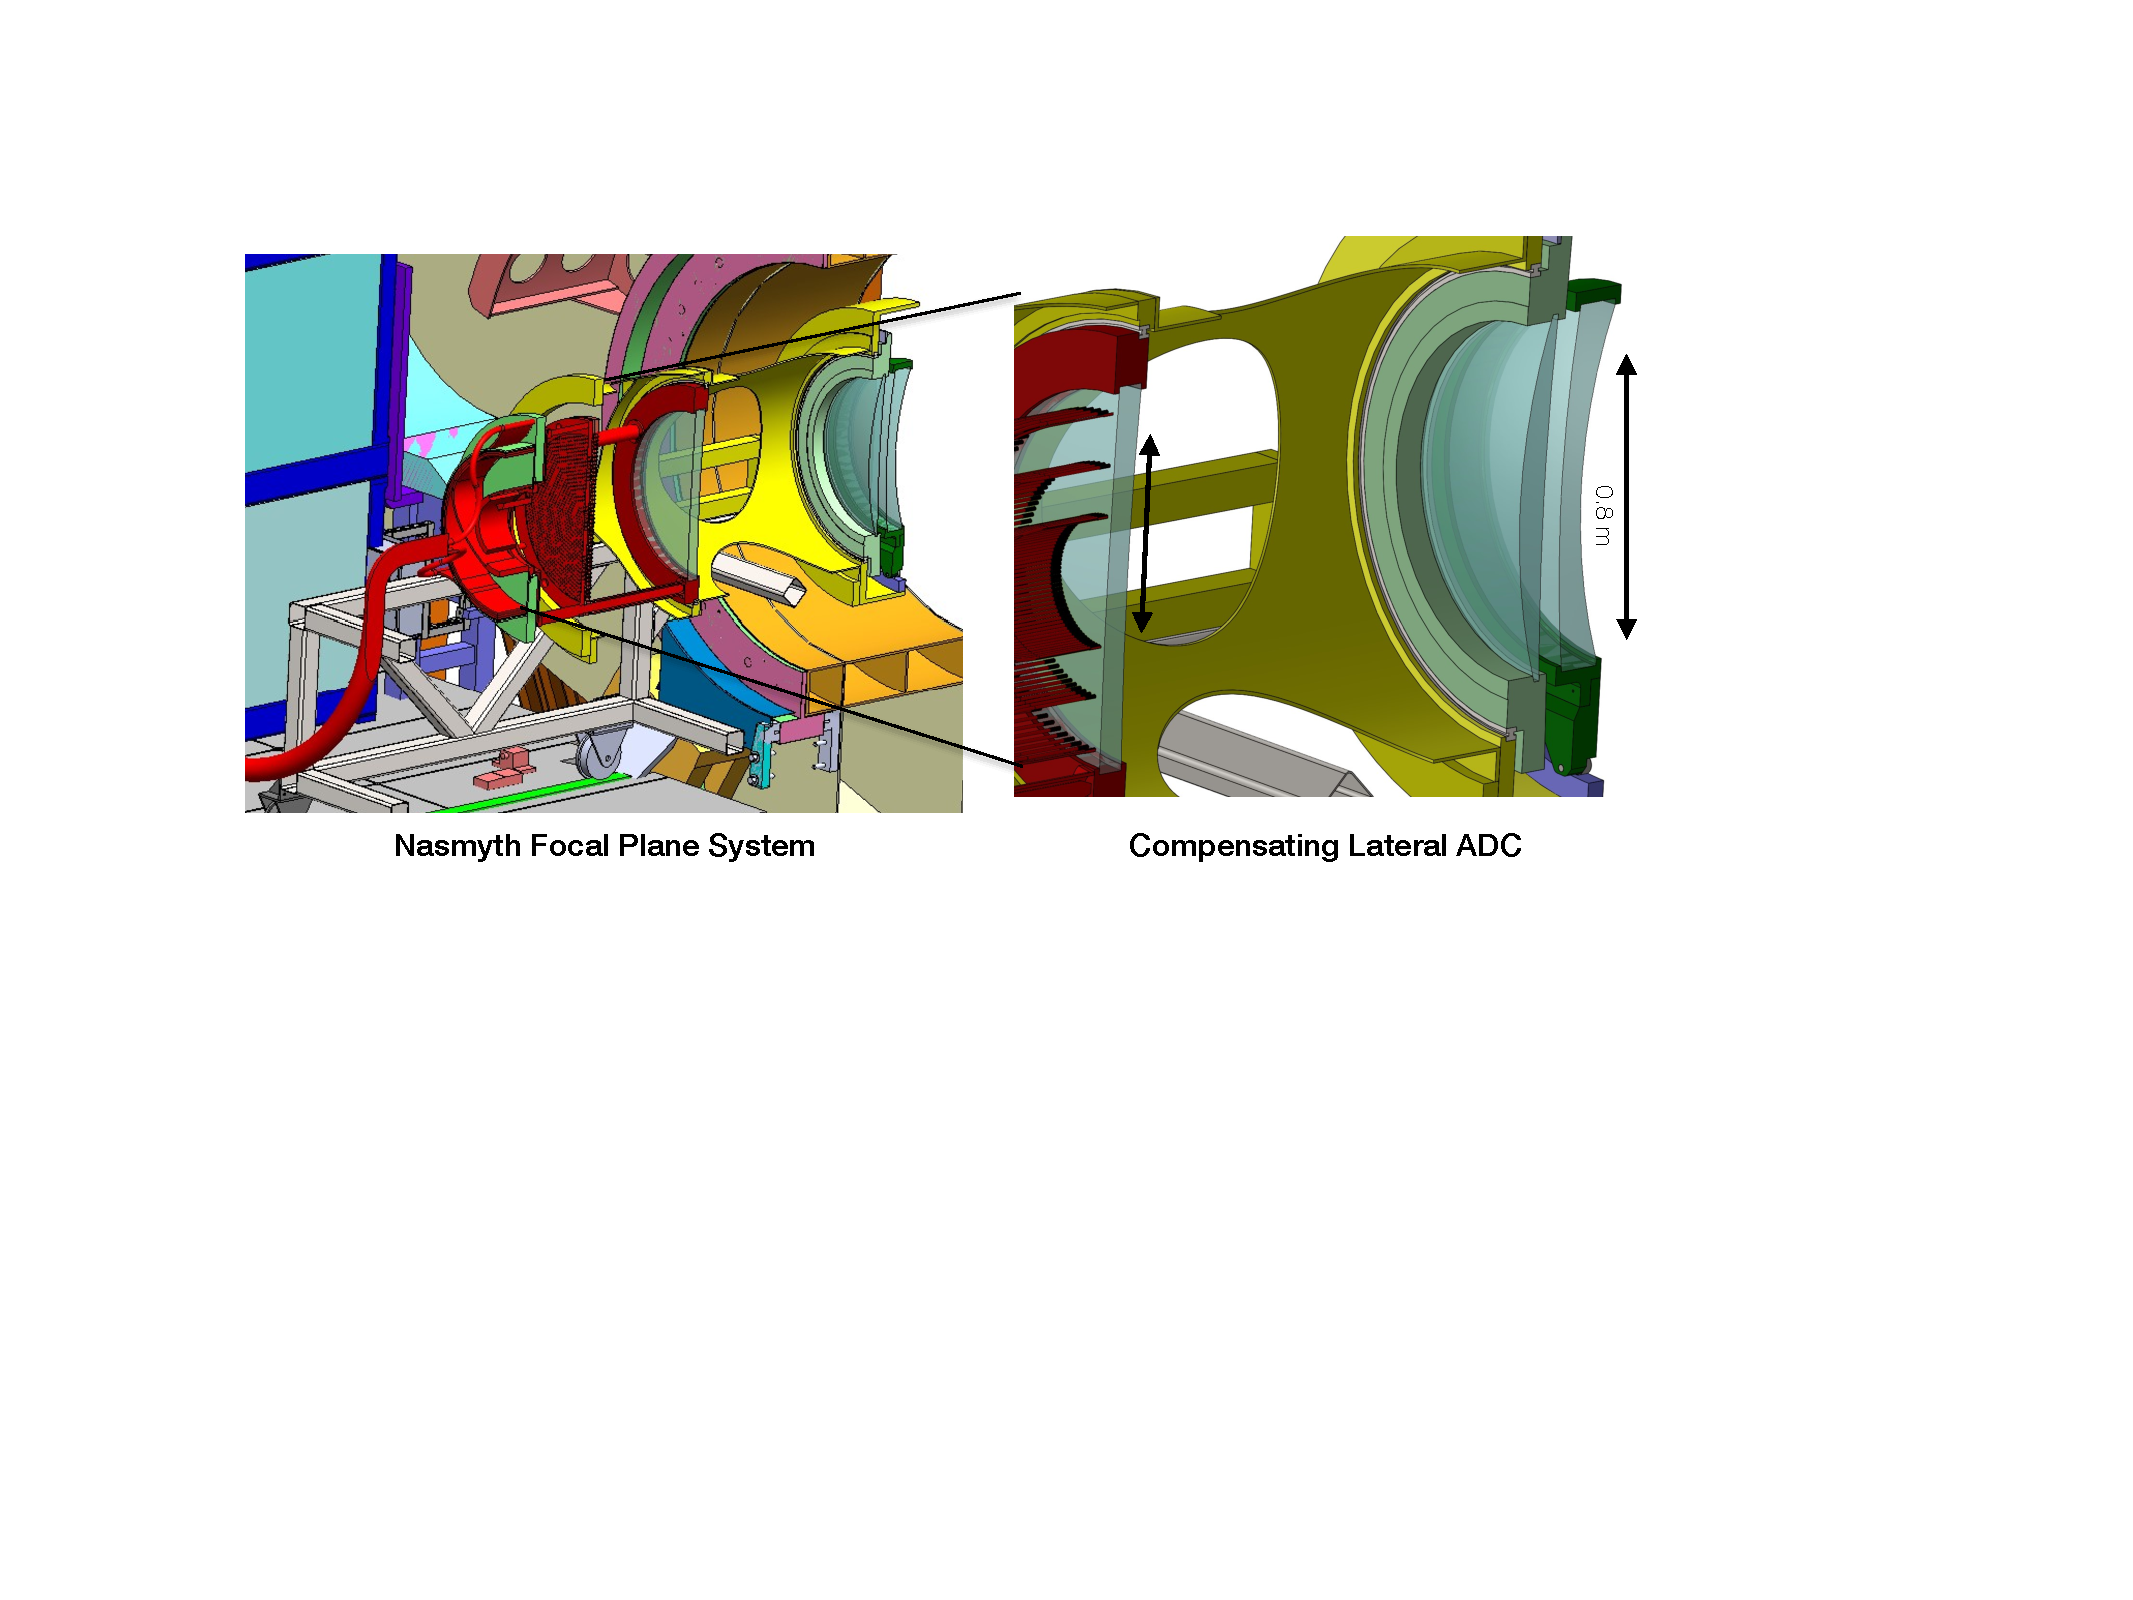
\includegraphics[width=0.8\textwidth]{figs/FOBOS_FocalPlane_v2.pdf}
\caption{\small {\it
Left}: Rendering of FOBOS focal plane system deployed at the Keck II
Nasmyth port. {\it Right}: Rendering of the ADC and focal surface with
Starbugs mounted (red cylinders).}
\label{fig:focalplane}
\end{figure}
%%%%%%%%%%%%%%%%%%%%%%%%%%%%%%%%%%%%%%%%%%%%%%%%%%%%%%%%%%%%%%%%%%%%%%%%

\section{Technical Description}
\label{sec:concept}
% \noindent \comment{1 page}

% Here's an alternative way to put in figures if we want captions on the side (to save space)
% Could introduce a new ``counter'' to count and label figures appropriately
%\centerline{\hbox{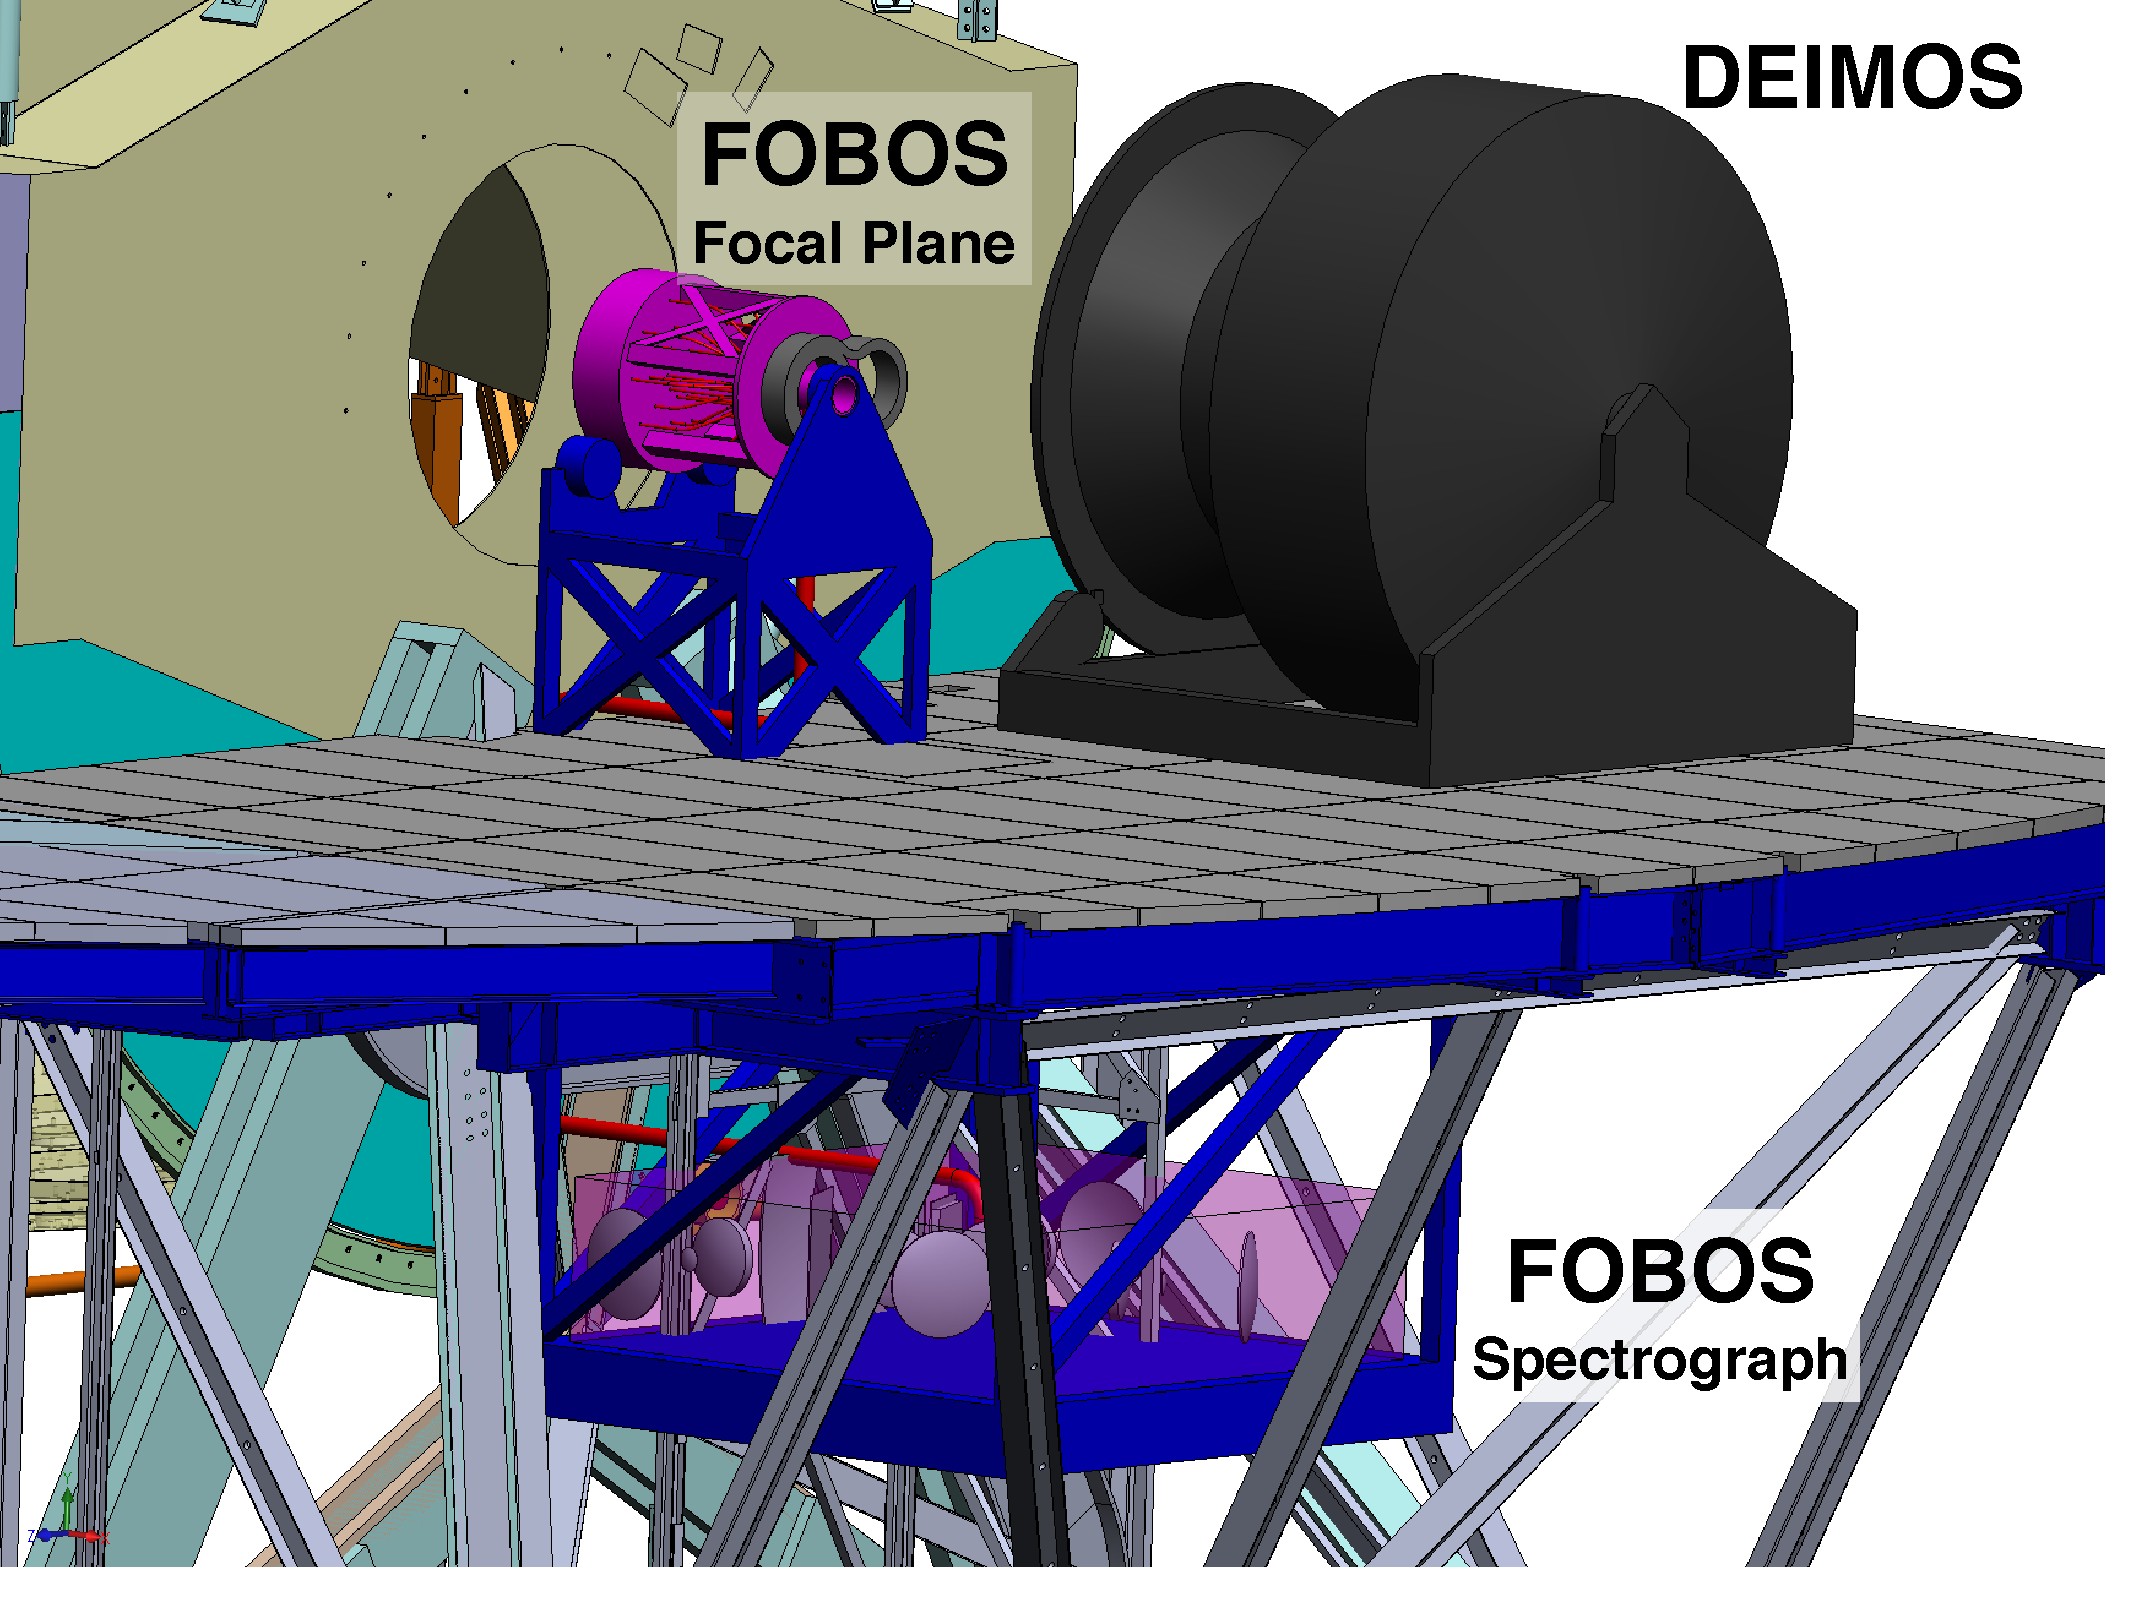
\includegraphics[width=0.6\textwidth, angle=0]{figs/FOBOSatKeck_v1.pdf}
%    \hspace{0.1cm} \vspace{2in}
%    \parbox[b]{0.3\textwidth}{\small {\bf Figure ??:} Rendering of FOBOS instrument systems deployed at the Keck II Nasmyth port.  By mounting the FOBOS spectrographs under the Nasmyth platform, other instruments like DEIMOS can maintain access to the telescope. \vspace{2cm}}}}

Mounted at the Nasmyth focus of Keck II Telescope at WMKO, FOBOS will
be one of the most powerful spectroscopic facilities deployed in the
next decade. FOBOS includes a compensating lateral atmospheric
dispersion corrector (CLADC; Fig.~\ref{fig:focalplane}) to ensure
that target light from all wavelengths falls on allocated fibers
while also correcting image aberrations at the edges of the 20~arcmin
diameter Keck field. Each of the CLADC lenses is $\sim$700~mm in
diameter, the first two are closely spaced with lateral relative
motions of element one supplied by a single axis of motion acting
along a curve equal to the radius of curvature of the first lens
surface (1028~mm). The total offset of this lens is rather small at
$\sim1$00~mm. The final CLADC lens translates by $\sim$50~mm and
tilts slightly to track the focal-plane shift. This last element acts to
correct the telecentricity error into the fiber system and acts as the
drive surface for the Starbug positioning system.
Starbugs patrol a large on-sky area ($\sim$3~arcmin), enabling
flexible and dynamic targeting configurations with adjacent fibers as
close as 10~arcsec.

% Reni- Can you check my numbers on the CLADC motion? - NKM
% How much do we go into risks?  How about this - NKM

Starbugs, first proposed in 2004 \citep{2004SPIE.5495..600M}, and
later perfected by AAO for use on TAIPAN \citep{2016SPIE.9912E..1WS}
are a truly remarkable fiber-positioning system. They move by {\it
walking} on the focal plane using a pair of piezo tube actuators. A
weak vacuum adheres the Starbugs to the surface of the field plate
and provides the frictional normal forces needed to allow for the
walking action of the piezo tubes. Positional feedback is provided by
way of a camera imaging back-illuminated fibers on the focal plane.
This system allows for a highly configurable focal plane both in
terms of target densities and configuration of the fibers within an
individual actuator. The Starbug payload can be both a single fiber or
fiber-bundle IFU. The TAIPAN instrument,
currently on sky conducting a large galaxy survey, is the proving ground
for the readiness of this technology. It is worth noting that,
although Starbugs are our preferred and baseline positioning
technology, no aspect of FOBOS's current front-end design precludes
using a zonal system, such as those used for MOONS, PFS, or DESI. The
last element of the CLADC can be eliminated and replaced with a zonal
actuator bed that conforms to the focal plane shape. Telecentricity
can be maintained by alignment of the actuator axis to the incoming
beam as is currently being designed for the SDSS-V robotic
focal-plane system.

A total of 1800 fibers with 150-$\mu$m core diameter are deployed at the curved focal plane. Microlens fore-optics
convert the f/15 Keck input beam to a faster f/3.2 focal ratio, which both demagnifies the entrance aperture
($\approx$0.9$^{\prime\prime}$ diameter) and allows for a better coupling to the fiber numerical aperture that
minimizes losses from focal ratio degradation (FRD).  With the IFU mode deployed, a different set of lenslet array
fore-optics would more finally sample the focal plane ($\approx$0.33$^{\prime\prime}$.  Accounting for 100 individual
sky fibers and 10 7-fiber flux calibration bundles, 25 science IFUs, each comprised of 61 fibers, would deploy in this
mode.  The diameter of each 61-fiber bundle corresponds to 3$^{\prime\prime}$ on-sky.  A single 61-fiber bundle would remain fixed at the field center in all FOBOS observing modes, enabling rapid target acquisition of transient sources.

The focal-plane plate rotates and translates to follow image
positions as the telescope tracks across the sky. The fiber run is
kept as short as possible to maintain high throughput at UV
wavelengths (a 10~m Polymicro Silica fiber transmits $\sim$70\% and
$\sim$85\% of light at 310~nm and 350~nm, respectively). Special care
is given to stress-relief cabling to minimize instabilities (e.g.,
variable FRD) over the fiber run. To maintain the highest possible
transition efficiency there are no connectors used within the fiber
run. When FOBOS is not in use, the focal-plane unit detaches from the
front-end, ADC module and its associated robotics, and it is stored
with the spectrographs on the Nasmyth platform. This allows the ADC
module to be transferred to any of the instrument park positions. All
other Keck-II instruments can still be used without modification.

%%%%%%%%%%%%%%%%%%%%%%%%%%%%%%%%%%%%%%%%%%%%%%%%%%%%%%%%%%%%%%%%%%%%%%%%
\begin{figure}[h!]
\vskip -0.1in
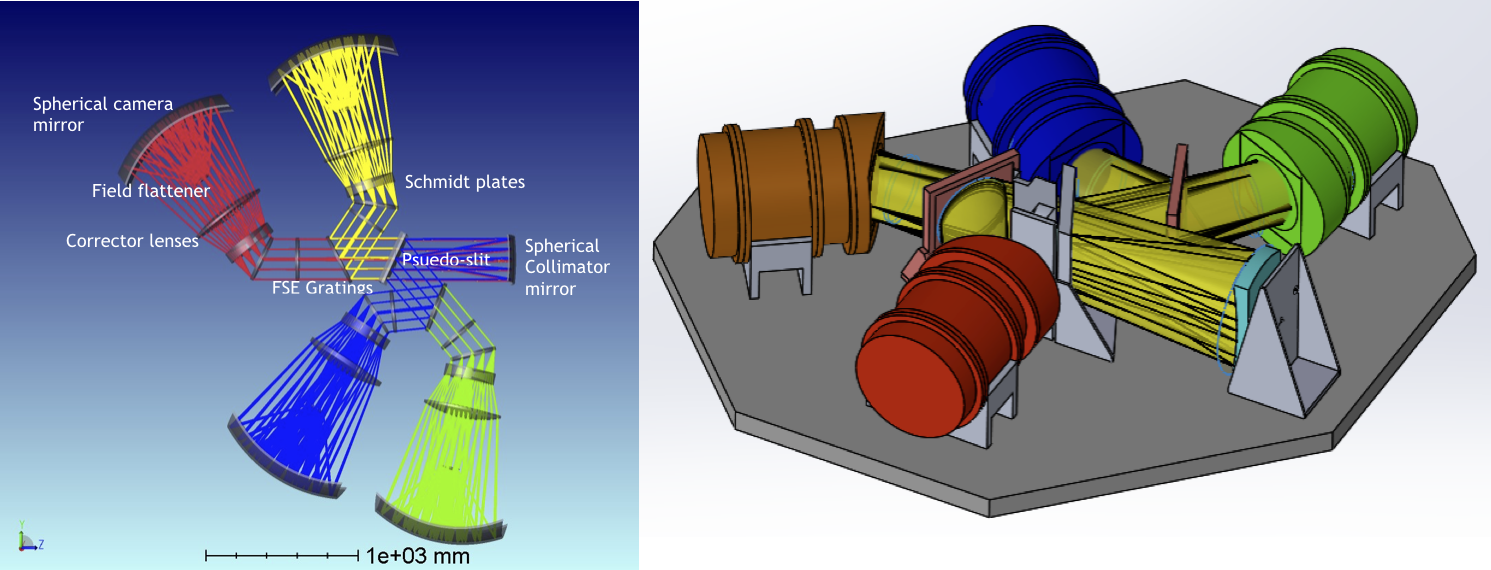
\includegraphics[width=0.96\textwidth]{figs/FOBOS_spec_optical-CAD.png}
\caption{\small Optical design (left) and mechancial rendering (right) of a 4-channel FOBOS spectrograph employing catadioptric cameras.
Light from a 600-fiber pseudo-slit strikes a collimating mirror and then
passes back through subsequent dichroics before entering each grating-camera unit.}
\label{fig:spectrograph}
\end{figure}
%%%%%%%%%%%%%%%%%%%%%%%%%%%%%%%%%%%%%%%%%%%%%%%%%%%%%%%%%%%%%%%%%%%%%%%%

FOBOS's three identical spectrographs (Fig.~\ref{fig:spectrograph})
are each fed by a pseudoslit of 600 fibers. Each FOBOS spectrograph
uses a series of dichroics to divide the 259~mm collimated beam into
four wavelength channels, providing an instantaneous broad-band
coverage from 0.31--1 $\mu$m. Fused-silica etched (FSE) gratings
provide mid-channel spectral resolutions of $R\sim3500$ at high
diffraction efficiency in each channel. The dispersed light is
focused by an f/1.1 catadioptric camera\footnote{Based on the camera
design for the Multi-Object Optical and Near-infrared Spectrograph
(MOONS) on the Very Large Telescope (VLT).} and recorded by an
on-axis 4k$\times$4k CCD mounted at the center of the first camera
lens element. Unlike the mountable ADC module, the spectrographs are
housed in a permanent temperature-controlled structure on the Nasmyth
deck. The end-to-end instrument throughput peaks at 60\% and is
greater than 30\% at {\it all} wavelengths.

FOBOS will include observatory level systems for precise instrument
calibration using dome-interior screen illumination, a metrology system
for accurate fiber positioning, and guide cameras for field acquisition
and guiding.  Initial deployment of the focal-plane will focus on a
single-fiber format, with a secondary deployment of multi-format fiber
bundles.  Beyond FOBOS, future instruments could share the focal plane, integrating their
fiber feeds to separate spectrographs optimized for higher spectral resolution, and/or
different wavelengths (e.g., the near-IR).  FOBOS is ideal for taking full advantage of a future
Ground-Layer Adaptive Optics capability.  It also allows for testing advances in spectrometer design that may be critical to future spectroscopic facilities.



%%%%
% -- Proposed Work and Budget
% --     FOBOS Keck White Paper 2019
%%%%

% ========================================================================
% - leverage experience from Shane prime focus ADC; Harland design; Matt
%   Radovan may know; Dave Cowley probably best person to talk to

\subsection{Technology Drivers}
\label{sec:design}

FOBOS will provide key capabilities in the near-term thanks to
deployment at the existing Keck II telescope. It both carries a
relatively modest cost compared to other proposed large-scale
spectroscopic facilities (e.g., MSE, SpecTel) and helps lay the
groundwork for their realization. Thus, while FOBOS will prove to be
a valuable long-term investment for the W.~M.~Keck Observatory, it
can also provide for invaluable technological development leading to
efficiency and cost-cutting strategies for these larger facilities.

\subsubsection{Starbugs fiber positioners} Starbugs are a positioning
technology developed and deployed by Australian Astronomical Optics
(AAO), which has partnered with our team to generate a conceptual
design for use of Starbugs by FOBOS. The Starbugs positioning systems
is highly attractive because of its flexibility. This flexibility is
both in terms of configuring a given set of fiber, as well as the
prospect of exchanging different groups of Starbugs with different
payloads and/or those that feed different spectrographs (e.g., high
vs.\ low resolution). With such a flexible focal plane deployment,
FOBOS can serve as a platform for cost-cutting technology
development, which is not possible with fixed-format instruments like
PFS and DESI. Starbugs are currently being tested on-sky with the
TAIPAN instrument at the UK Schmidt Telescope and published results
on their performance are expected in summer 2019.

\subsubsection{Spectrograph Cost} \comment{to edit} Here we make the
case that FOBOS is a platform for figuring out how to build future
dedicated spectroscopic telescopes like SpecTel cheaper.

\subsubsection{Data Systems} A key to FOBOS's success with the
development of robust data-reduction and data-analysis pipelines,
building on the heritage of efforts within SDSS, DESI, and MaNGA. In
particular, the FOBOS data-analysis pipeline (DAP) will take
advantage of the fixed spectral format and common target classes to
provide high-level data products, including Doppler shifts,
emission-line strengths, and template continuum fits (cf., Westfall
et al.; SDSS-IV MaNGA DAP). Planning will include development of
user-friendly platforms built on the Keck Observatory Archive for
serving raw data, reduced spectra, and DAP science products.

% \comment{to edit/remove} We will develop the requirements and initial
% concept for the FOBOS data simulator following instrument
% forward-modeling techniques developed by DESI. The simulator will
% enable tests of potential FOBOS science cases (e.g., exposure time
% estimates, redshifting success). For the MSIP proposal, we will
% construct a detailed plan for evolving the data simulator into
% data-reduction and data-analysis pipelines.

\subsection{Current Status} FOBOS is currently in its conceptual
design phase, building from a down-selection process as one of the
designs for the Wide-Field Optical Spectrograph for TMT. Recently,
FOBOS has been awarded Phase-A funding by WMKO Observatory, receiving
the full endorsement of the Keck Science Steering Committee. These
funds are devoted building out the conceptual design in preparation
for future funding proposals, particularly the NSF MSIP and MsRI
calls.

\subsection{Cost Estimates} \comment{Nick M.}

% \noindent \textbf{Operations:} Powered by Starbugs fiber positioners,
% FOBOS will enable fast ($<$2 minute), dynamic reallocation of fibers. We will
% develop an initial target allocation simulator to determine
% efficiencies for various science programs and explore options for
% program combination and optimization under different observing
% scenarios. This work requires planning interfaces with the fiber
% positioning control software and the Keck user.


% To efficiently
% determine the best options given a wide range of possible targets and
% desired observing outcomes, we will develop a conceptual design for
% MAISTRO,\footnote{MAISTRO: Modular Artificial Intelligence System for
% Target Reallocation and Observing.} an ``artificial intelligence''
% (AI) targeting system that will learn optimization strategies for
% assigning targets from a database of overlapping observing programs
% with pre-defined priorities. The AI package will aggregate data
% quality using a quick-look reduction package, science-driven
% performance metrics, {\it and real-time assessments of the observing
% conditions} to make dynamic targeting recommendations. For example,
% if conditions are slightly less than optimal, MAISTRO would
% reconfigure Starbugs to brighter objects in a field or implement a
% different program prioritization. MAISTRO will incorporate updated
% target lists and priorities from the active observer and could easily
% be over-ridden at any time. Fractions of the full FOBOS multiplex
% might also be reserved ``manual targeting'' as required by the
% program PI.

%   - maintains a database with observational progress on individual
%     targets in the survey and
%   - dynamically reallocates fibers based on real-time assessments of
%     the aggregate S/N of each target to meet the specific need of each
%     science case.

% This requires significant design and testing of a combined software
% package and hardware interface.  Specific considerations involve (1)
% fast and robust reduction procedures (cf. MaNGA DOS) that can assess
% the aggregate data and (2) a responsive database with a schema
% optimized for real-time decision making to select targets for
% (re)acquisition while accounting for collision limitations.  Provided
% enough design effort, this lends itself to a machine-learning
% application.




% \pagebreak
\clearpage
\begin{multicols}{2}
\scriptsize
\bibliographystyle{apj}
\bibliography{references}
\end{multicols}

% \textbf{References}



\end{document}
